\documentclass[a4paper,titlepage]{article}
\usepackage{hyperref}
\usepackage{graphicx}
\usepackage{dingbat}
\usepackage{fancyhdr}
\usepackage{geometry}
\geometry{left=3.0truecm,right=3.0truecm,top=3.0truecm,bottom=3.0truecm} 

\author{David Acreman}
\title{Profiling Firedrake for the APinTA-PDEs project}

\begin{document}
\pagestyle{fancy}
\lhead{}
\chead{}
\rhead{Profiling report}

\maketitle
\pagebreak
\tableofcontents
\pagebreak

%%%%%%%%%%%%%%%%%%%%%%%%%%%%%%%%%%%%%%%%%%%%%%%%%%%%%%%%%%%%%%%%%%%%%%%%%%%%%%%%%%%%%%%%%%%%%%%%%%%%%%%%%%%%%%%%%%%%%%%%%%%%%%%%%%%%%%

\section*{To do}

\begin{enumerate}
\item Add server information to table~\ref{tab:software}
\item Write up ITAC examples
\item Builds on Isca: GCC reference, platform optimised Intel toolchain. Describe how to use Easybuild to set up the Intel build if this works.
\item (Firedrake example on Isca)
\item Add examples using ARM MAP
\item Firedrake example with Performance Reports and MAP
\item Add examples using Cray PAT perftools-lite
\item Describe other capabilities of Cray PAT in addition to perftools-lite including rank re-ordering
\item Write conclusions and recommendations section: include the next steps e.g. how to switch to reference BLAS/Lapack to test the impact of maths libraries
\end{enumerate}

\pagebreak

%%%%%%%%%%%%%%%%%%%%%%%%%%%%%%%%%%%%%%%%%%%%%%%%%%%%%%%%%%%%%%%%%%%%%%%%%%%%%%%%%%%%%%%%%%%%%%%%%%%%%%%%%%%%%%%%%%%%%%%%%%%%%%%%%%%%%%

\section{Introduction}

In order to understand the performance characteristics of numerical schemes and the impact of potential optimisations it is necessary to gather information beyond simple measures of elapsed run times. A number of profiling tools exist which are capable of gathering performance information from applications parallelised using MPI, for example the time spent in MPI calls and the identification of performance problems such as load imbalance. This document gives an overview of the profiling tools available to the APinTA-PDEs project with a focus on tools which can provide information about MPI and related performance issues. 

The domain specific language Firedrake will be used extensively for development work in the course of the project. Firedrake is python-based and uses code generation, and these characteristics makes integrating Firedrake with profilers more complex than for traditional HPC applications written using C/C++ and/or Fortran which are compiled then run. Although this report primarily focusses on Firedrake the profiling tools evaluated could be used for profiling other codes used by the project even if those tools are not currently suitable for use with Firedrake.

Section~\ref{section:target_platforms} presents the target platforms being considered in this report and reviews the hardware and software available on these systems. Section~\ref{section:test_cases} describes the test cases which will be used to demonstrate the profilers. The profiling tools available to the project are discussed in section \ref{section:profiling_tools} and their capabilities demonstrated with the examples from section~\ref{section:test_cases}. Section~\ref{section:builds} discusses the successful builds of Firedrake on the target platforms and which profilers the builds can be used with. Proof-of-concept results from these profilers are shown in section~\ref{section:profiling_firedrake}. Finally section~\ref{section:conclusions} present conclusions and recommendations. 

%%%%%%%%%%%%%%%%%%%%%%%%%%%%%%%%%%%%%%%%%%%%%%%%%%%%%%%%%%%%%%%%%%%%%%%%%%%%%%%%%%%%%%%%%%%%%%%%%%%%%%%%%%%%%%%%%%%%%%%%%%%%%%%%%%%%%%

\section{Target platforms}
\label{section:target_platforms}

An overview of the hardware in the target platforms for this project is shown in Table~\ref{tab:hardware}. 
%
\begin{table}[htp]
\begin{center}
\begin{tabular}{|l|l|r|r|l|}
\hline 
System         & Processor        & Cores/node & Memory/node     & Interconnect \\
\hline
Archer-2       & AMD x86\_64         & 128        & 256 GB DRAM  & HPE Cray Slingshot  \\
Isambard XCI   & Thunder X2 ARM64    &  64        & 256 GB DRAM  & Cray Aries          \\
Isambard A64FX & Fujitsu A64FX ARM64 & 48         & 32 GB HBM    & Mellanox Infiniband \\
Isca           & Intel x86\_64       & 16/20      & 128 GB DRAM  & Mellanox Infiniband \\
Server         & AMD x86\_64         & 128        & 256 GB DRAM  & None                \\
\hline
\end{tabular}
\end{center}
\caption{Target platform hardware specifications. The Isambard A64FX platform has high bandwidth memory (HBM) which should give better performance than DRAM but has a smaller capacity.}
\label{tab:hardware}
\end{table}%
The target HPC platforms are Archer-2 (national tier-1), Isambard (national tier-2) and Isca (local tier-3). Isambard has two separate systems based on the ARM64 architecture: the XCI system which is an established production system, and the A64FX system which is a newer system. The A64FX system should be considered a stretch objective as the hardware and software are relatively new and less well tested. The project has purchased a local server which is designed to be similar to an Archer compute node, although it will run Ubuntu which will make it easier to build Firedrake. The server can function as a reference installation as it will use an unmodified Firedrake installation, rather than the more customised installations on the HPC platforms which will use non-standard components, for example MPI libraries and maths libraries.

An overview of the software stacks on the target platforms is shown in Table~\ref{tab:software}. 
\begin{table}[htp]
\begin{center}
\begin{tabular}{|l|l|l|l|l|}
\hline 
System         & Compilers               & MPI libraries  & Maths lib.       & Profilers  \\
\hline
Archer-2       & Cray, GNU, AOCC         & Cray MPICH2     & Cray libsci     & Cray      \\
Isambard XCI   & Cray, GNU, ARM          & Cray MPICH2     & Cray libsci     & Cray, ARM \\
Isambard A64FX & Cray, GNU, ARM, Fujitsu & Cray MVAPICH2   & Cray libsci     & ARM       \\
Isca (GCC)     & GNU                     & OpenMPI         & OpenBLAS        & None      \\
Isca (Intel)   & Intel                   & Intel           & Intel MKL       & Intel     \\
Server         & GNU                     & MPICH?          & ???             & None      \\
\hline
\end{tabular}
\end{center}
\caption{Software stacks on target platforms. AOCC is the AMD Optimizing Compiler Collection. Intel MPI and MVAPICH are MPICH derivatives which support an Infiniband interconnect.
The Cray profiler is Cray Performance Analysis Tools (PAT), the ARM profilers are part of the ARM Forge tool suite and the Intel profilers are part of the Intel Parallel Studio suite.
The A64FX system did not appear to have a perftools module.}
\label{tab:software}
\end{table}
Each HPC platform has the GNU compilers, a compiler from the processor vendor (AMD, Intel, ARM and Fujitsu) and Cray systems also have the Cray compiler\footnote{On Isambard A64FX run \texttt{module use /lustre/software/aarch64/modulefiles} to make extra modules available}. The GNU compilers are the one compiler family which is available on all the target platforms.

On the Cray systems compilation is handled by wrapper scripts from the Cray Programming Environment. The wrapper script can run different compilers depending on which programming environment module is loaded at compile time (e.g. if \texttt{PrgEnv-cray} is loaded then \texttt{cc} calls the Cray C compiler and if \texttt{PrgEnv-gnu} is loaded \texttt{cc} calls the GNU C compiler). The MPI library and maths library (Cray libsci) are then linked by the wrapper script. On Cray systems the standard profiling tool is Cray Performance Analysis Tools (PAT) but on Isambard the profiling tools from the ARM Forge suite\footnote{ARM Forge was previously known as Allinea Forge} are also available.

The software environment on Isca is managed using Easybuild which has the concept of a toolchain. There are two toolchains on Isca: the GCC-foss toolchain and the Intel toolchain. Each toolchain has a different MPI library and maths library. Intel Parallel Studio has an MPI profiling tool called Intel Trace Analyzer and Collector (ITAC) which needs to use Intel MPI. However the Intel toolchain can be used with GNU compilers such that the Intel MPI library wrapper scripts call the GNU compilers; the wrapper script \texttt{mpiicc} is the MPI-enabled wrapper for the Intel C compiler with Intel MPI, whereas \texttt{mpicc} is the MPI-enabled wrapper for the GNU C compiler with Intel MPI. Hence is it possible to use the GNU compilers with the Intel MPI library which allows profiling with Intel Trace Analyzer and Collector. 

The server does not currently have any profiling software but Intel's Parallel Studio product is now available for free download as part of the HPC toolkit from the newer OneAPI product\footnote{\url{https://software.intel.com/content/www/us/en/develop/tools/oneapi/all-toolkits.html}}. There is also the option of obtaining an evaluation licence for ARM Forge to test these tools on the server.

%%%%%%%%%%%%%%%%%%%%%%%%%%%%%%%%%%%%%%%%%%%%%%%%%%%%%%%%%%%%%%%%%%%%%%%%%%%%%%%%%%%%%%%%%%%%%%%%%%%%%%%%%%%%%%%%%%%%%%%%%%%%%%%%%%%%%%

\section{Test cases}
\label{section:test_cases}

The profilers will be tested using three different versions of a Mandelbrot set calculation. The different versions parallelise the calculation in different ways and have different performance characteristics:
\begin{itemize}
\item Version 1: divides the computational domain into equal sized chunks along the real axis. This introduces a load imbalance.
\item Version 2: similar to version 1 but interleaves the iterations on the real axis to fix the load balance. This version (and version 1) pack a 2D array into a 1D buffer which is communicated using an \verb+MPI_Reduce+ and constitutes an overhead.
\item Version 3: implements a manager-worker pattern for distributing the iterations to ensure load balancing. This replaces the \verb+MPI_Reduce+ with point-to-point communication between the manager-process and the worker processes. One process (the manager process) does not perform any calculations which adversely affects performance with small numbers of MPI processes. However this version scales better to larger numbers of MPI processes.
\end{itemize}

The following tests will be used to demonstrate the profiling tools:
\begin{itemize}
\item Test 1: version 1, no I/O, 4 MPI processes
\item Test 2: version 1, with I/O, 4 MPI processes
\item Test 3: version 2, no I/O, 4 MPI processes
\item Test 4: version 3, no I/O, 4 MPI processes
\item Test 5: version 3, no I/O, 16 MPI processes 
\end{itemize}
These examples show the load imbalance vs. overhead (version 1 vs. version 2) and can the difference between collectives and point-to-point communication (version 2 vs version 3). The I/O is performed by writing to an ASCII file which causes a substantial overhead compared to the case without I/O.

%%%%%%%%%%%%%%%%%%%%%%%%%%%%%%%%%%%%%%%%%%%%%%%%%%%%%%%%%%%%%%%%%%%%%%%%%%%%%%%%%%%%%%%%%%%%%%%%%%%%%%%%%%%%%%%%%%%%%%%%%%%%%%%%%%%%%%

\section{Profiling tools}
\label{section:profiling_tools}

Within Firedrake itself performance information can be obtained from PETSc by adding the \verb+-log_view+ flag when running Firedrake. There is also the ability to time sections of code by adding a PyOP2 timed stage. These options will be available on all platforms when Firedrake is the target application but the rest of this report will look at how external profilers can be used to obtain extra information. There are external profilers already installed on the target platforms with different platforms having different profiling tool available:
%
\begin{itemize}
\item ARM Forge (currently only licensed on Isambard)
\item Intel Parallel Studio (Intel MPI only)
\item Cray PAT (Cray systems only)
\end{itemize}
%
Each of these products is a suite of tools and this report will focus on the tools appropriate for understanding the performance of MPI applications.

%---------------------------------------------------------------------------------------------------------------------

\subsection{Intel Trace Analyzer and Collector}

The MPI profiler in Intel Parallel Studio is called Intel Trace Analyzer and Collector (ITAC). Other profiling tools are available which provide information node-level performance.

In this example the Mandelbrot executable will be build with MPI tracing enabled. Firstly load the modules for the Intel compilers and the ITAC tool. 
\begin{verbatim}
> module load intel/2017b
> module load itac/2017.1.024
\end{verbatim}
Then compile the executable with \texttt{-trace} flag:
\begin{verbatim}
> mpicc -trace -o mandelbrot mandelbrot_mpi.c
\end{verbatim}
The \texttt{intel} and \texttt{itac} modules need to be loaded in the job script but no other modifications are required to the job script. When the job runs a number of additional files are generated, including a file with a \texttt{.stf} extension which is the trace file.
The profiling output can be viewed opening the trace file with the Trace Analyzer GUI:
\begin{verbatim}
> traceanalyzer.bin mandelbrot_mpi.stf &
\end{verbatim}

\noindent
\textbf{Test 1:} 
Figure~\ref{fig:test1_ITAC_summary} (top) shows the opening summary page for test 1 (Mandelbrot version 1, no I/O, 4 MPI processes).
\begin{figure}[htbp]
\begin{center}
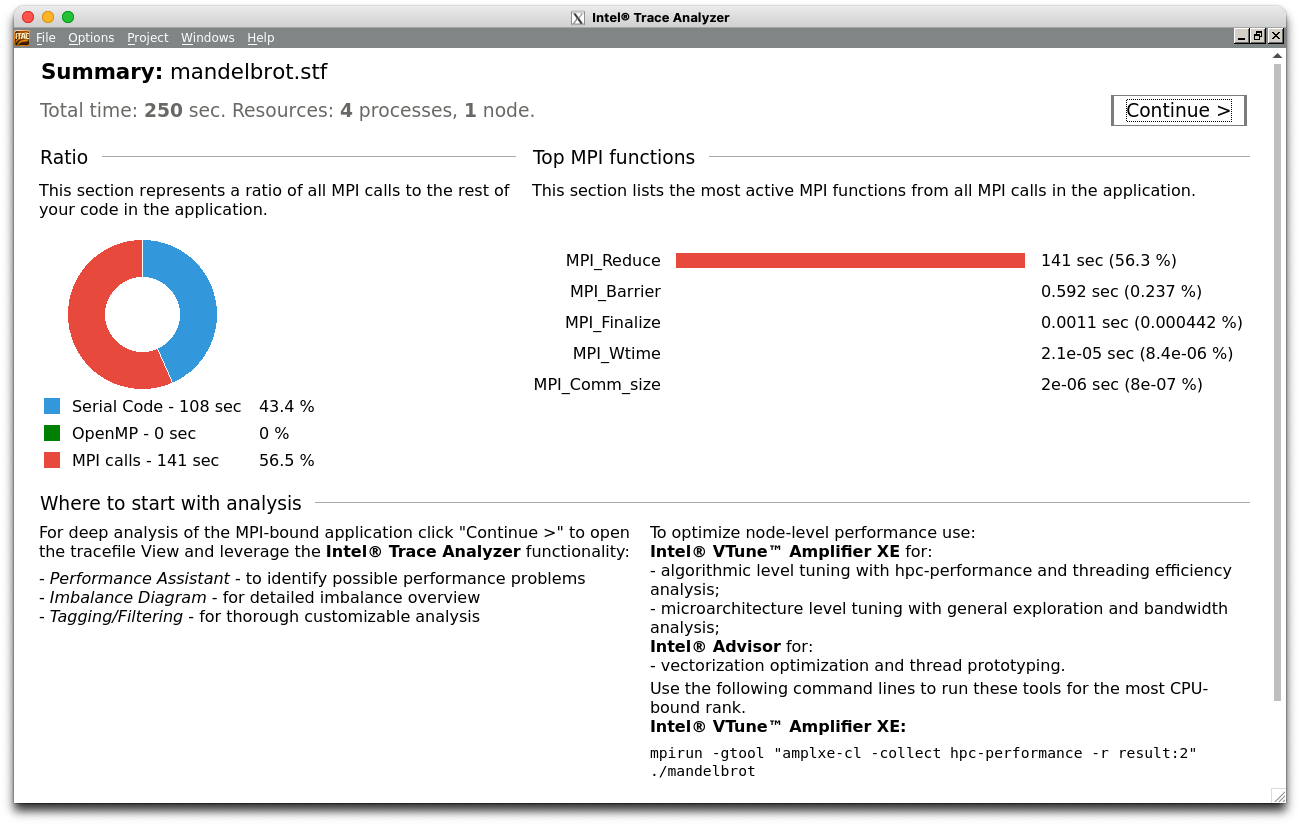
\includegraphics[scale=0.3]{figures/test1_summary}
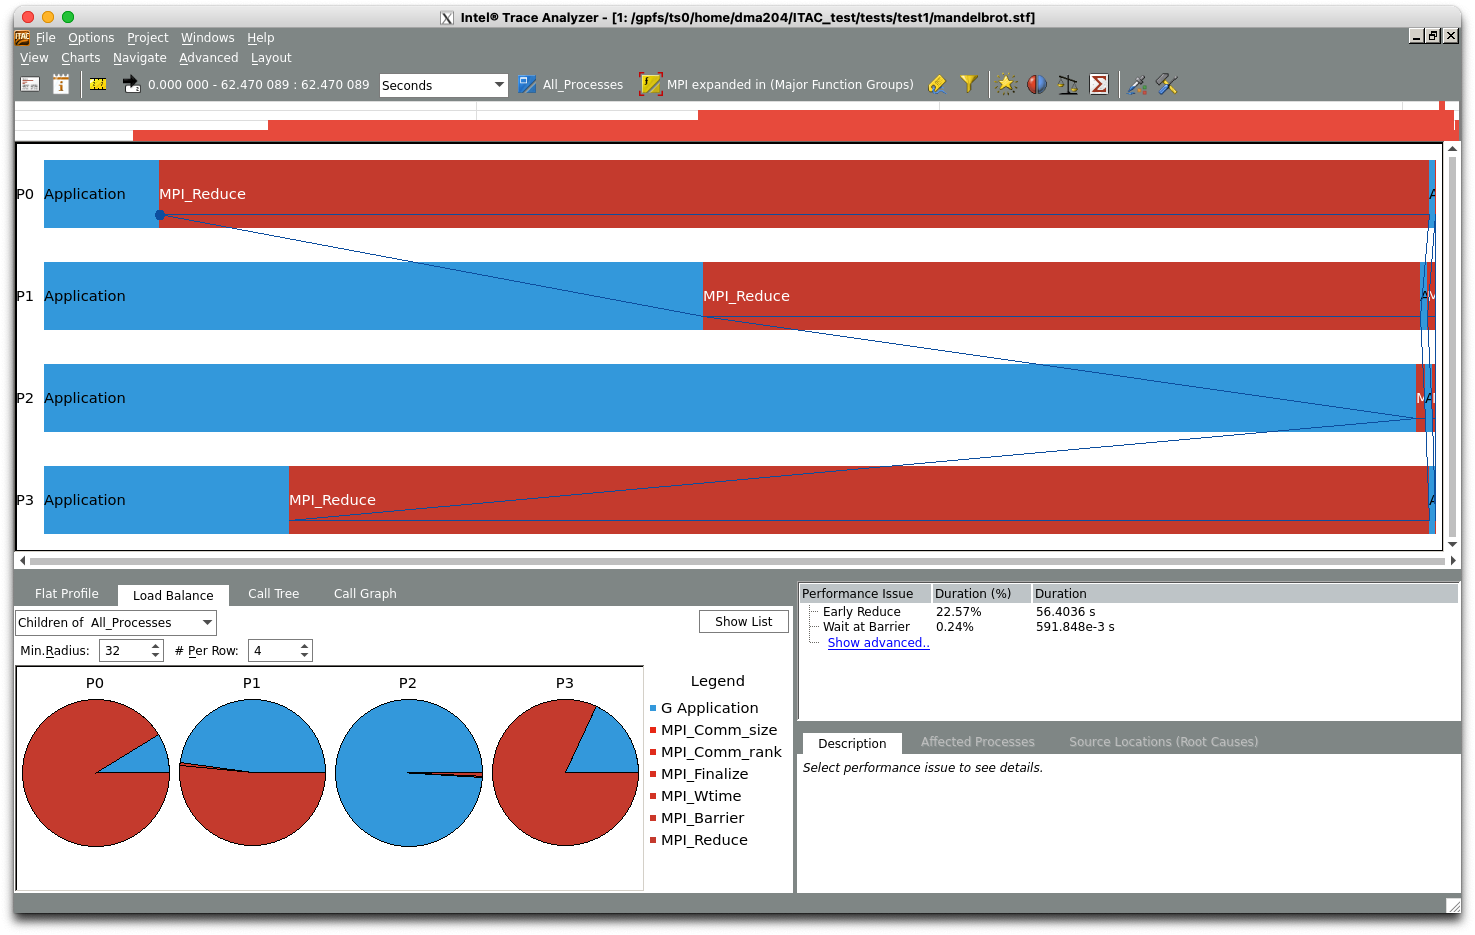
\includegraphics[scale=0.3]{figures/test1_eventTimeline}
\caption{Intel Trace Analyzer plots for test 1. On the summary page (top) the load imbalance shows up as a large fraction of time spent in \texttt{MPI\_Reduce}. The event timeline (bottom) shows that process 2 takes longer than the other processes to complete its iterations which results in the other processes waiting at the \texttt{MPI\_Reduce} call.}
\label{fig:test1_ITAC_summary}
\end{center}
\end{figure}
This test has a load imbalance which is seen as a large fraction of time spent in \texttt{MPI\_Reduce}. The reduce itself is not time consuming (all communication takes place on the same compute node) but this is the blocking collective where the MPI processes synchronise. This can be seen more clearly in the lower panel of figure~\ref{fig:test1_ITAC_summary} which shows the event timeline. To view the event timeline as seen in this figure:
\begin{itemize}
\item Click the continue button on the summary page
\item Select \texttt{Charts} $\rightarrow$ \texttt{Event Timeline} to open a new pane showing process activity over time.
\item In the lower left pane select the \texttt{Load Balance} tab and click the \texttt{Show pies} button. 
\item Right click on a red MPI section in the timeline and choose \texttt{Ungroup MPI} from the drop down menu
\end{itemize}
The timeline shows that process 2 is taking much longer to complete its than the other processes which has resulted in processes 0, 1 and 3 waiting at the \verb+MPI_Reduce+ call.


\noindent
\textbf{Test 2:} this test is similar to test 1 but has I/O enabled. The summary page (see figure~\ref{fig:test2_ITAC_summary}) shows a significantly longer runtime (450s vs. 250s) and significant time spent in \verb+MPI_Barrier+. 
\begin{figure}[htbp]
\begin{center}
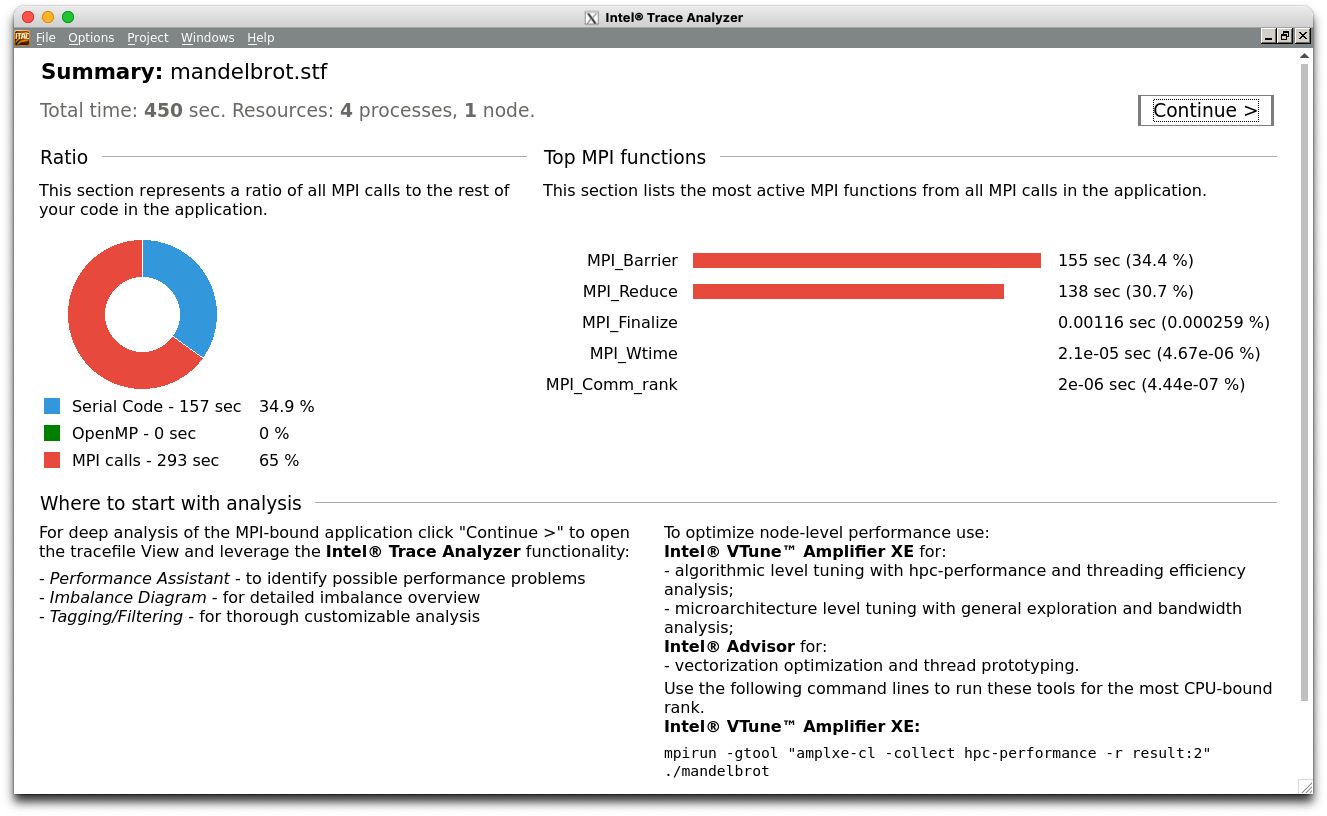
\includegraphics[scale=0.3]{figures/test2_summary}
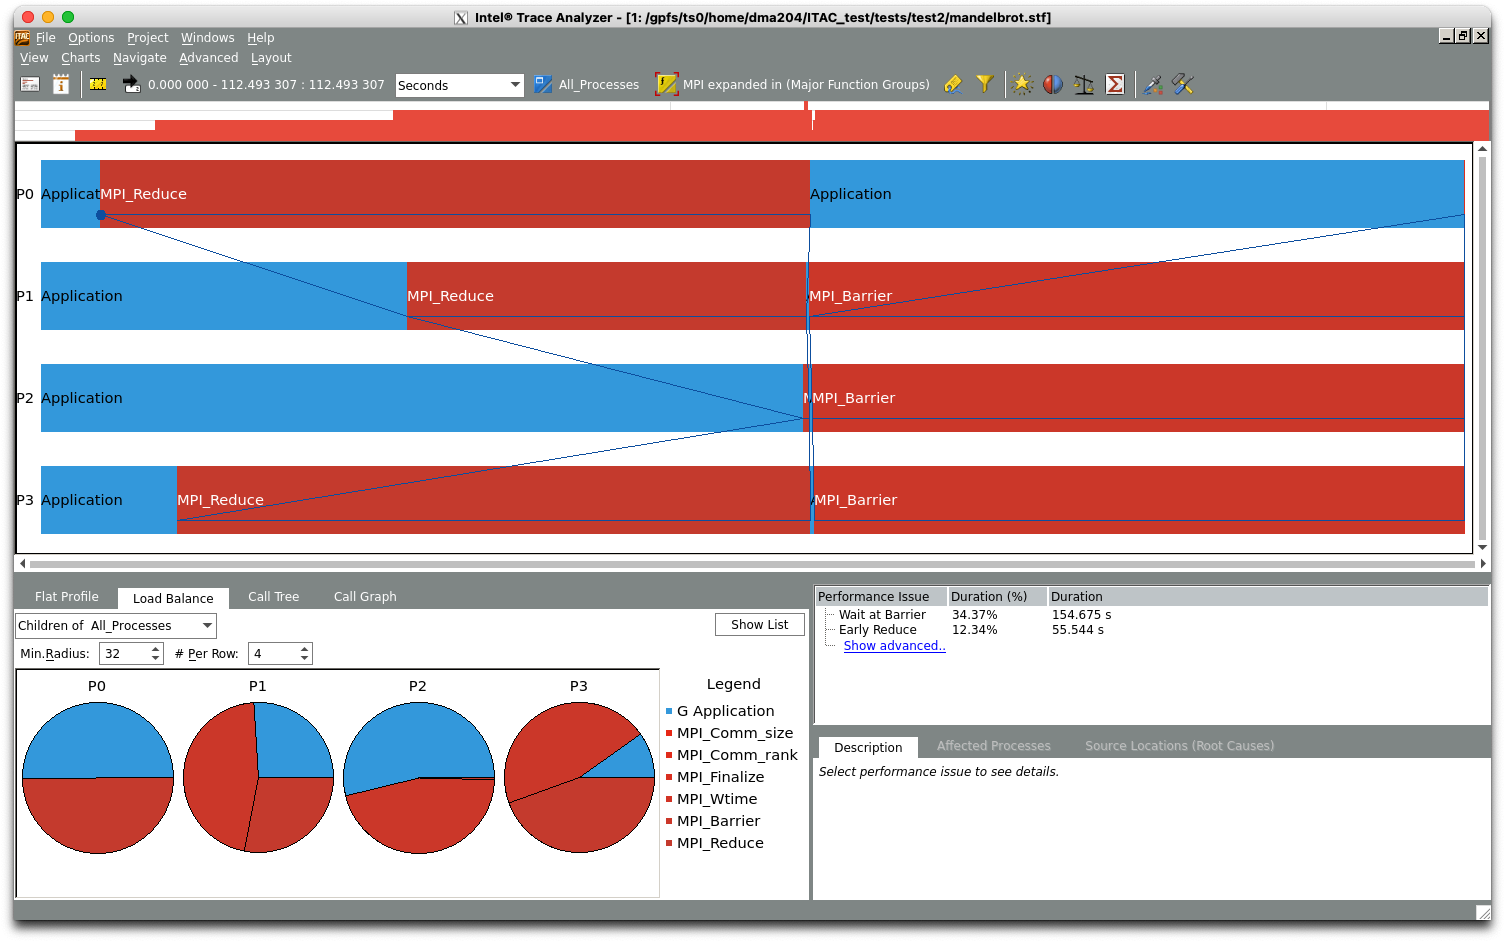
\includegraphics[scale=0.3]{figures/test2_eventTimeline}
\caption{Intel Trace Analyzer plots for test 2.}
\label{fig:test2_ITAC_summary}
\end{center}
\end{figure}
The I/O is carried by process 0 which causes all the other processes to wait at a barrier at the end of the program (processes are synchronised before a final run time is reported by process 0). The effect of switching on I/O has been to introduce another load imbalance, this time with process 0 working and all other processes waiting. This can be seen clearly in the timeline where there are two distinct phases both of which have a load imbalance, but is less clear from the summary or pie charts alone.

\noindent
\textbf{Test 3:}  
\begin{figure}[htbp]
\begin{center}
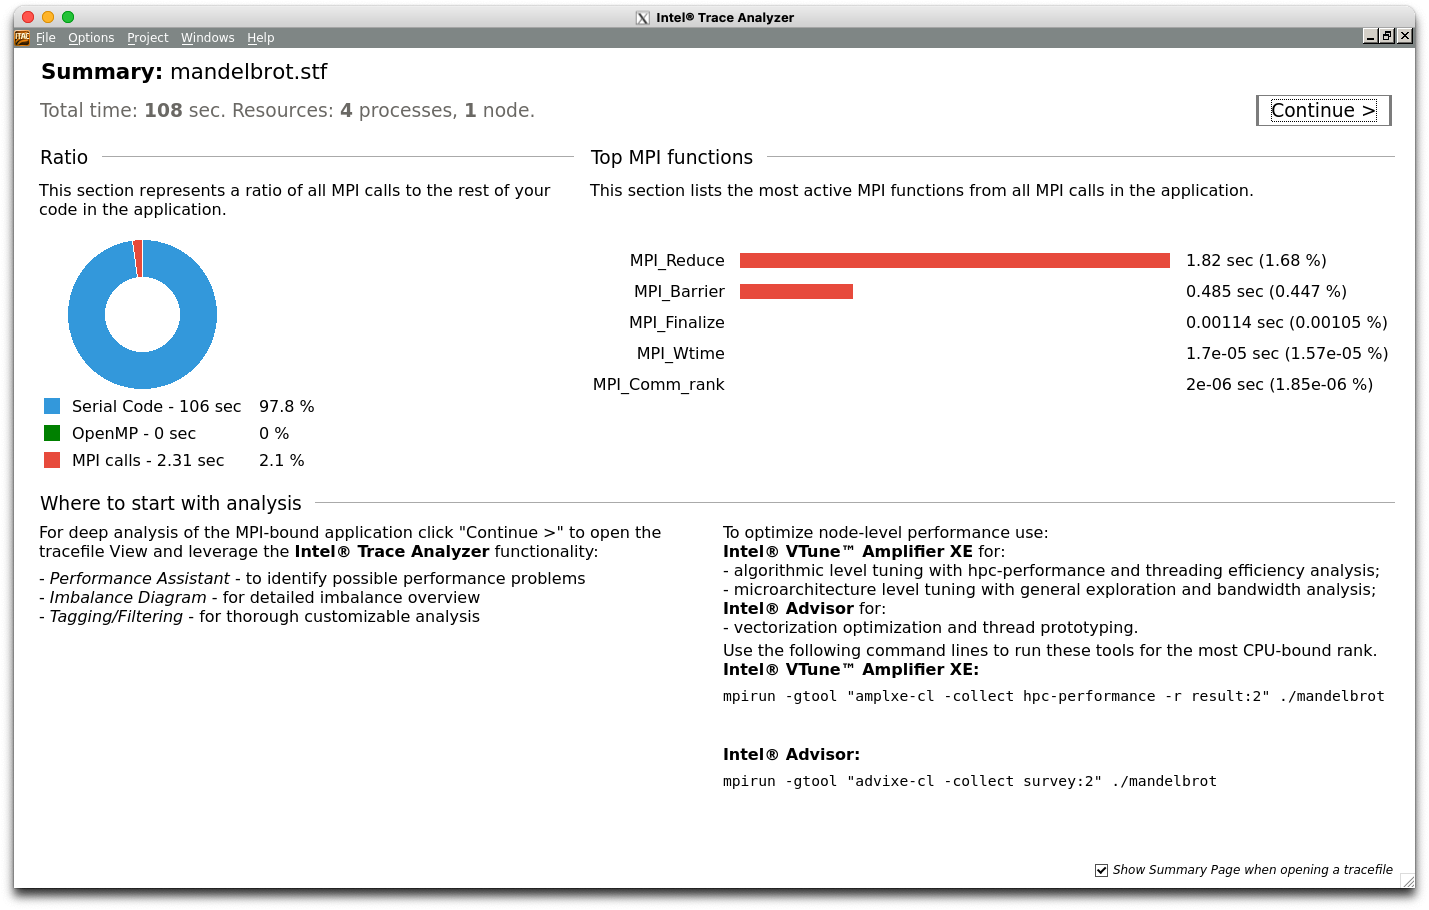
\includegraphics[scale=0.3]{figures/test3_summary}
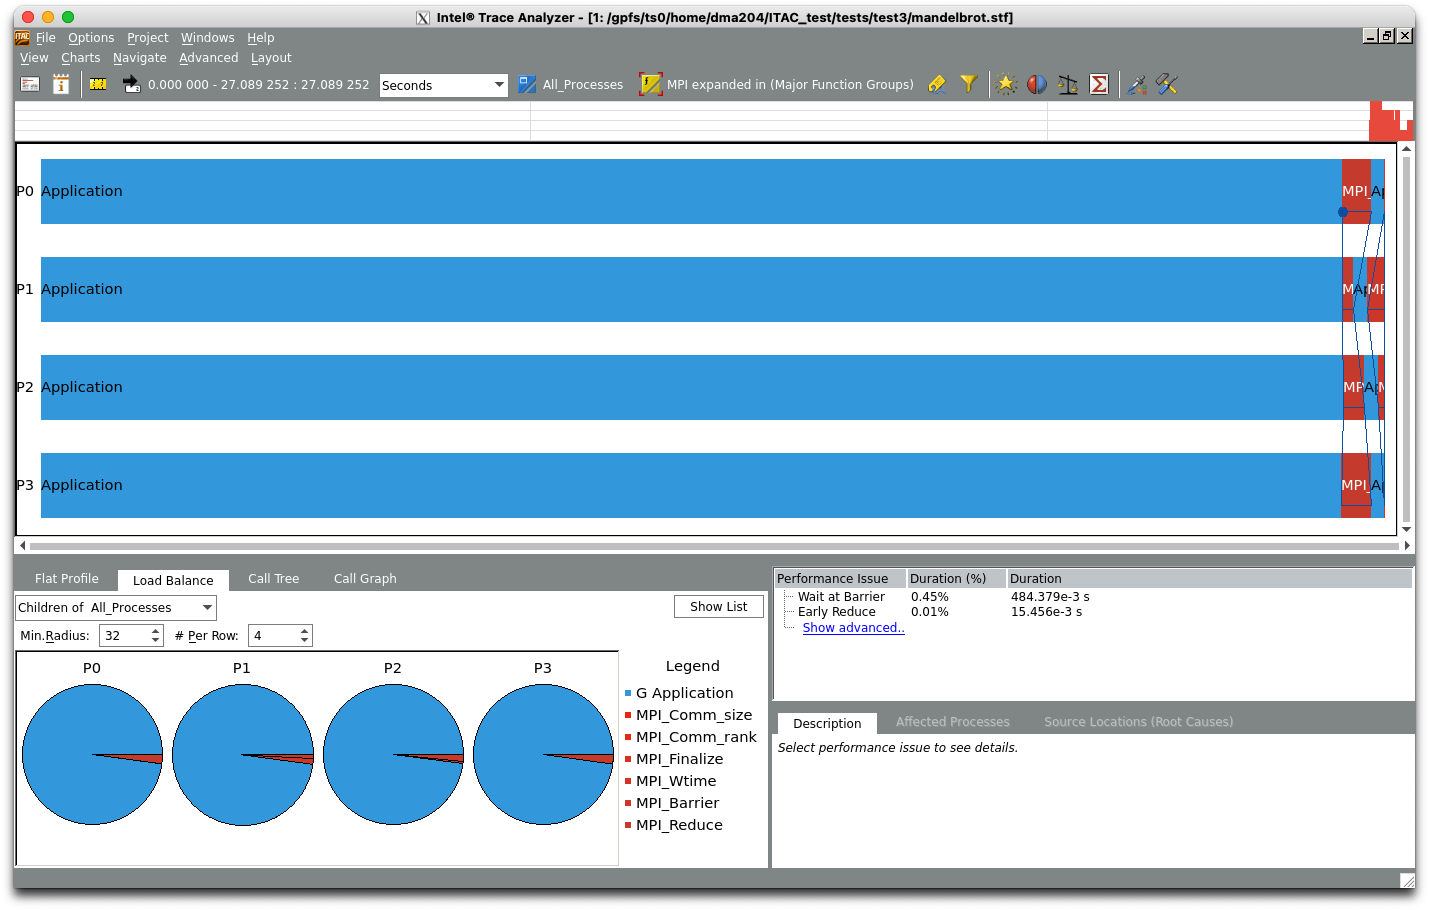
\includegraphics[scale=0.3]{figures/test3_eventTimeline}
\caption{Intel Trace Analyzer plots for test 3.}
\label{fig:test3_ITAC_summary}
\end{center}
\end{figure}

\noindent
\textbf{Test 4:}  \texttt{Charts} $\rightarrow$ \texttt{message profile}
\begin{figure}[htbp]
\begin{center}
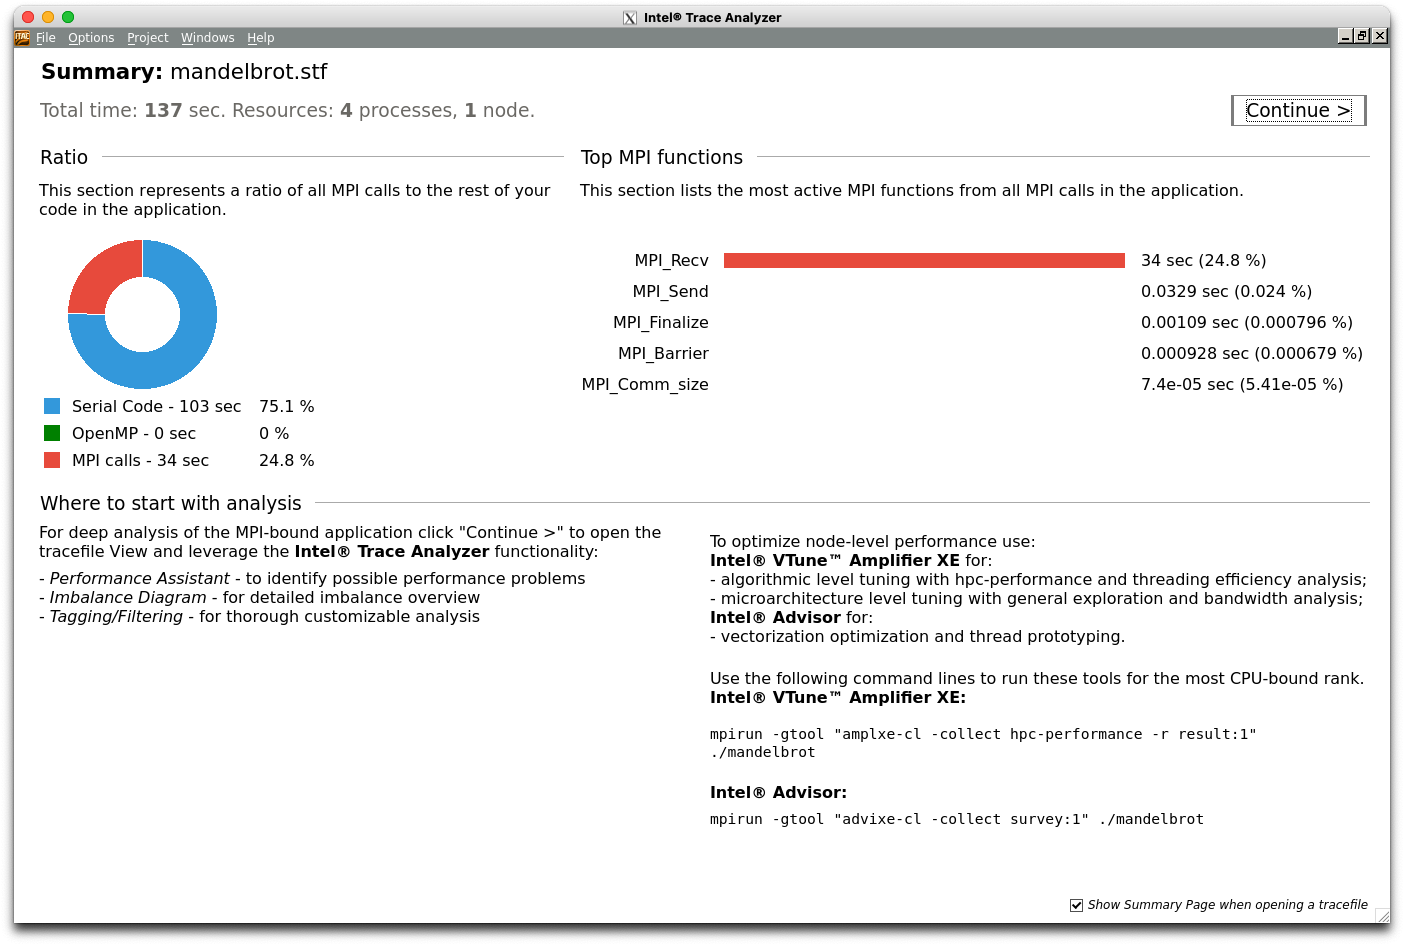
\includegraphics[scale=0.3]{figures/test4_summary}
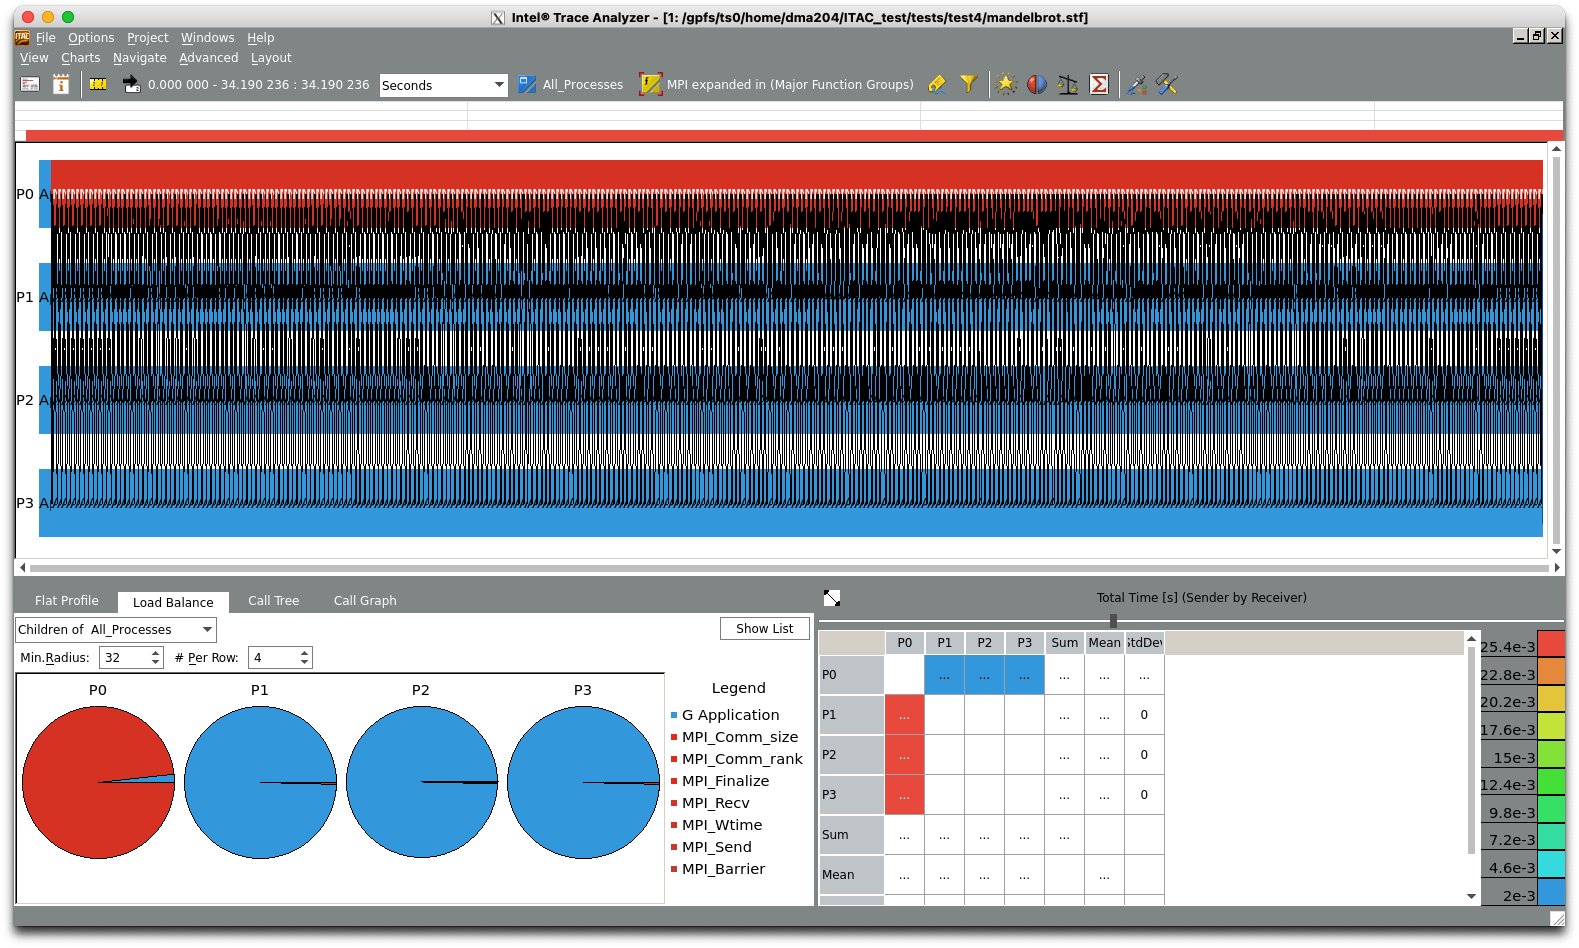
\includegraphics[scale=0.3]{figures/test4_eventTimeline}
\caption{Intel Trace Analyzer plots for test 4.}
\label{fig:test4_ITAC_summary}
\end{center}
\end{figure}

\noindent
\textbf{Test 5:}  
\begin{figure}[htbp]
\begin{center}
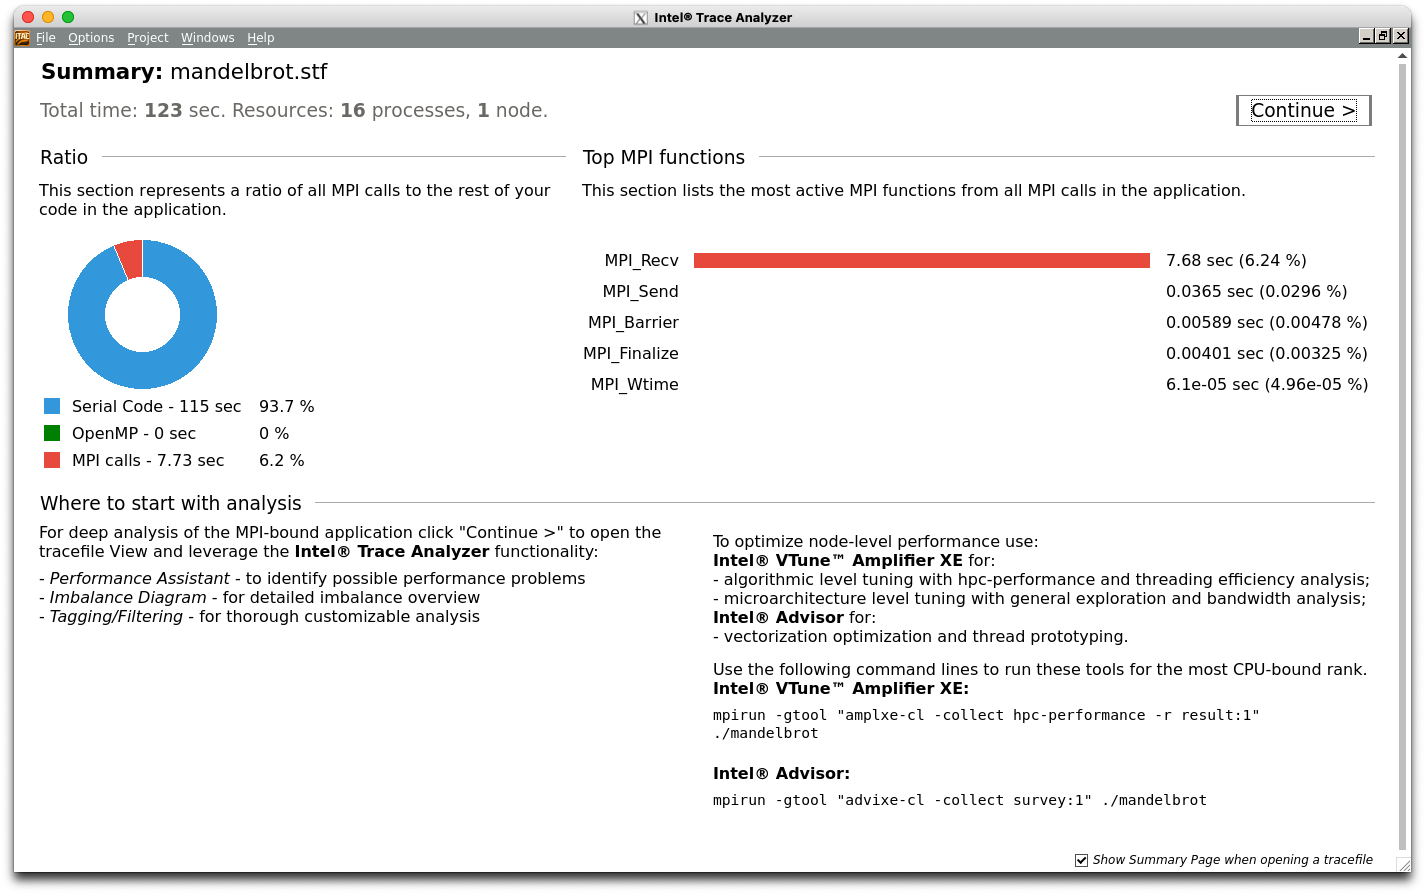
\includegraphics[scale=0.3]{figures/test5_summary}
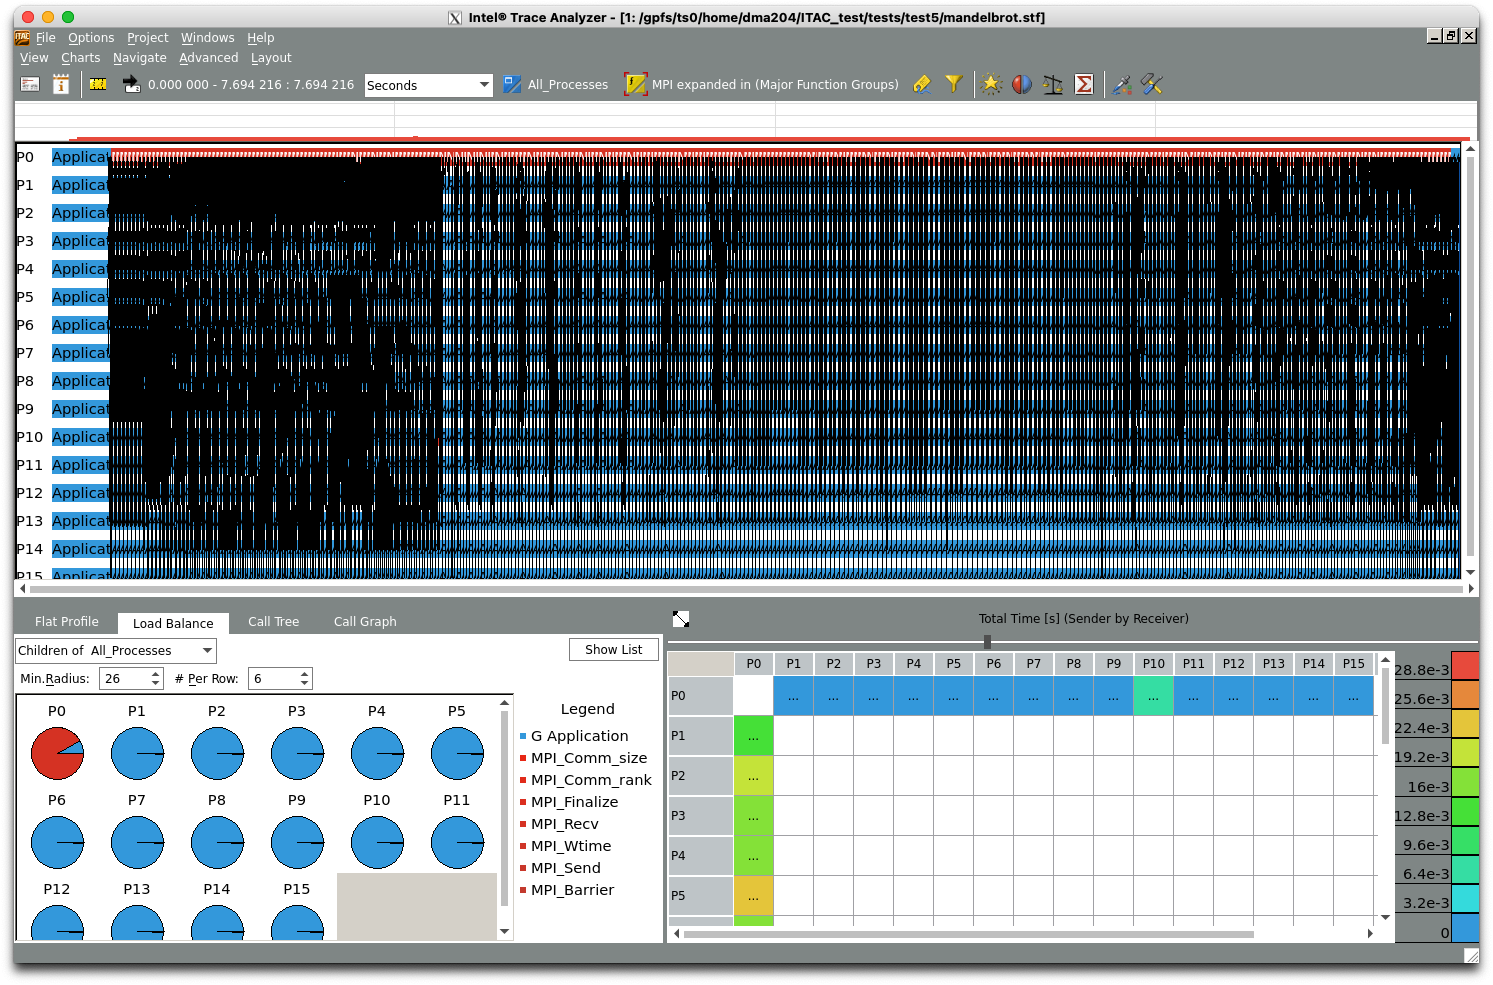
\includegraphics[scale=0.3]{figures/test5_eventTimeline}
\caption{Intel Trace Analyzer plots for test 5.}
\label{fig:test5_ITAC_summary}
\end{center}
\end{figure}

%---------------------------------------------------------------------------------------------------------------------

\subsection{ARM Forge}

The ARM Forge suite of development tools is available on the Isambard system. ARM Forge includes two performance tools: ``Performance Reports'' and ``MAP''. 
ARM MAP is a profiler which is part of the ARM Forge suite and it can profile C++, C, Fortran and Python\footnote{\url{https://www.arm.com/products/development-tools/server-and-hpc/forge/map}}.

%---

\subsubsection{Performance Reports}

The documentation for Performance Reports says that on Cray systems dynamic linking or explicit linking with the profiling libraries is required\footnote{\url{https://developer.arm.com/documentation/101136/2102/Performance-Reports/Get-started-with-Performance-Reports/Compile-on-Cray-X-series-systems}}. However in the latest Cray compilers dynamic linking is the default so no changes are required to the build process. The following shows an example session and output from Performance Reports on the Isambard XCI system.

No changes are required at compile time so simply compile the executable as normal. For this example the GCC compiler will be used:
\begin{verbatim}
> module switch PrgEnv-cray PrgEnv-gnu
> cc -o mandelbrot mandelbrot_mpi.c
\end{verbatim}
Two changes are required in the job script in order to activate performance reports. The first change is to load the \texttt{arm-forge} module:
\begin{verbatim}
module load tools/arm-forge
\end{verbatim}
and the second change is to add the \texttt{perf-report} command before the \texttt{aprun} command:
\begin{verbatim}
perf-report aprun -n ${nprocs} ./mandelbrot
\end{verbatim}
This method of launching a job under perf-report is referred to as Express Launch mode.
%
When the job runs two extra files are generated which contain the output from the performance report in text and HTML formats. The output from running a performance report on the Mandelbrot version 1 example using 4 MPI processes is shown in figure~\ref{fig:perf-report_MB1}.  
%
\begin{figure}[htbp]
\begin{center}
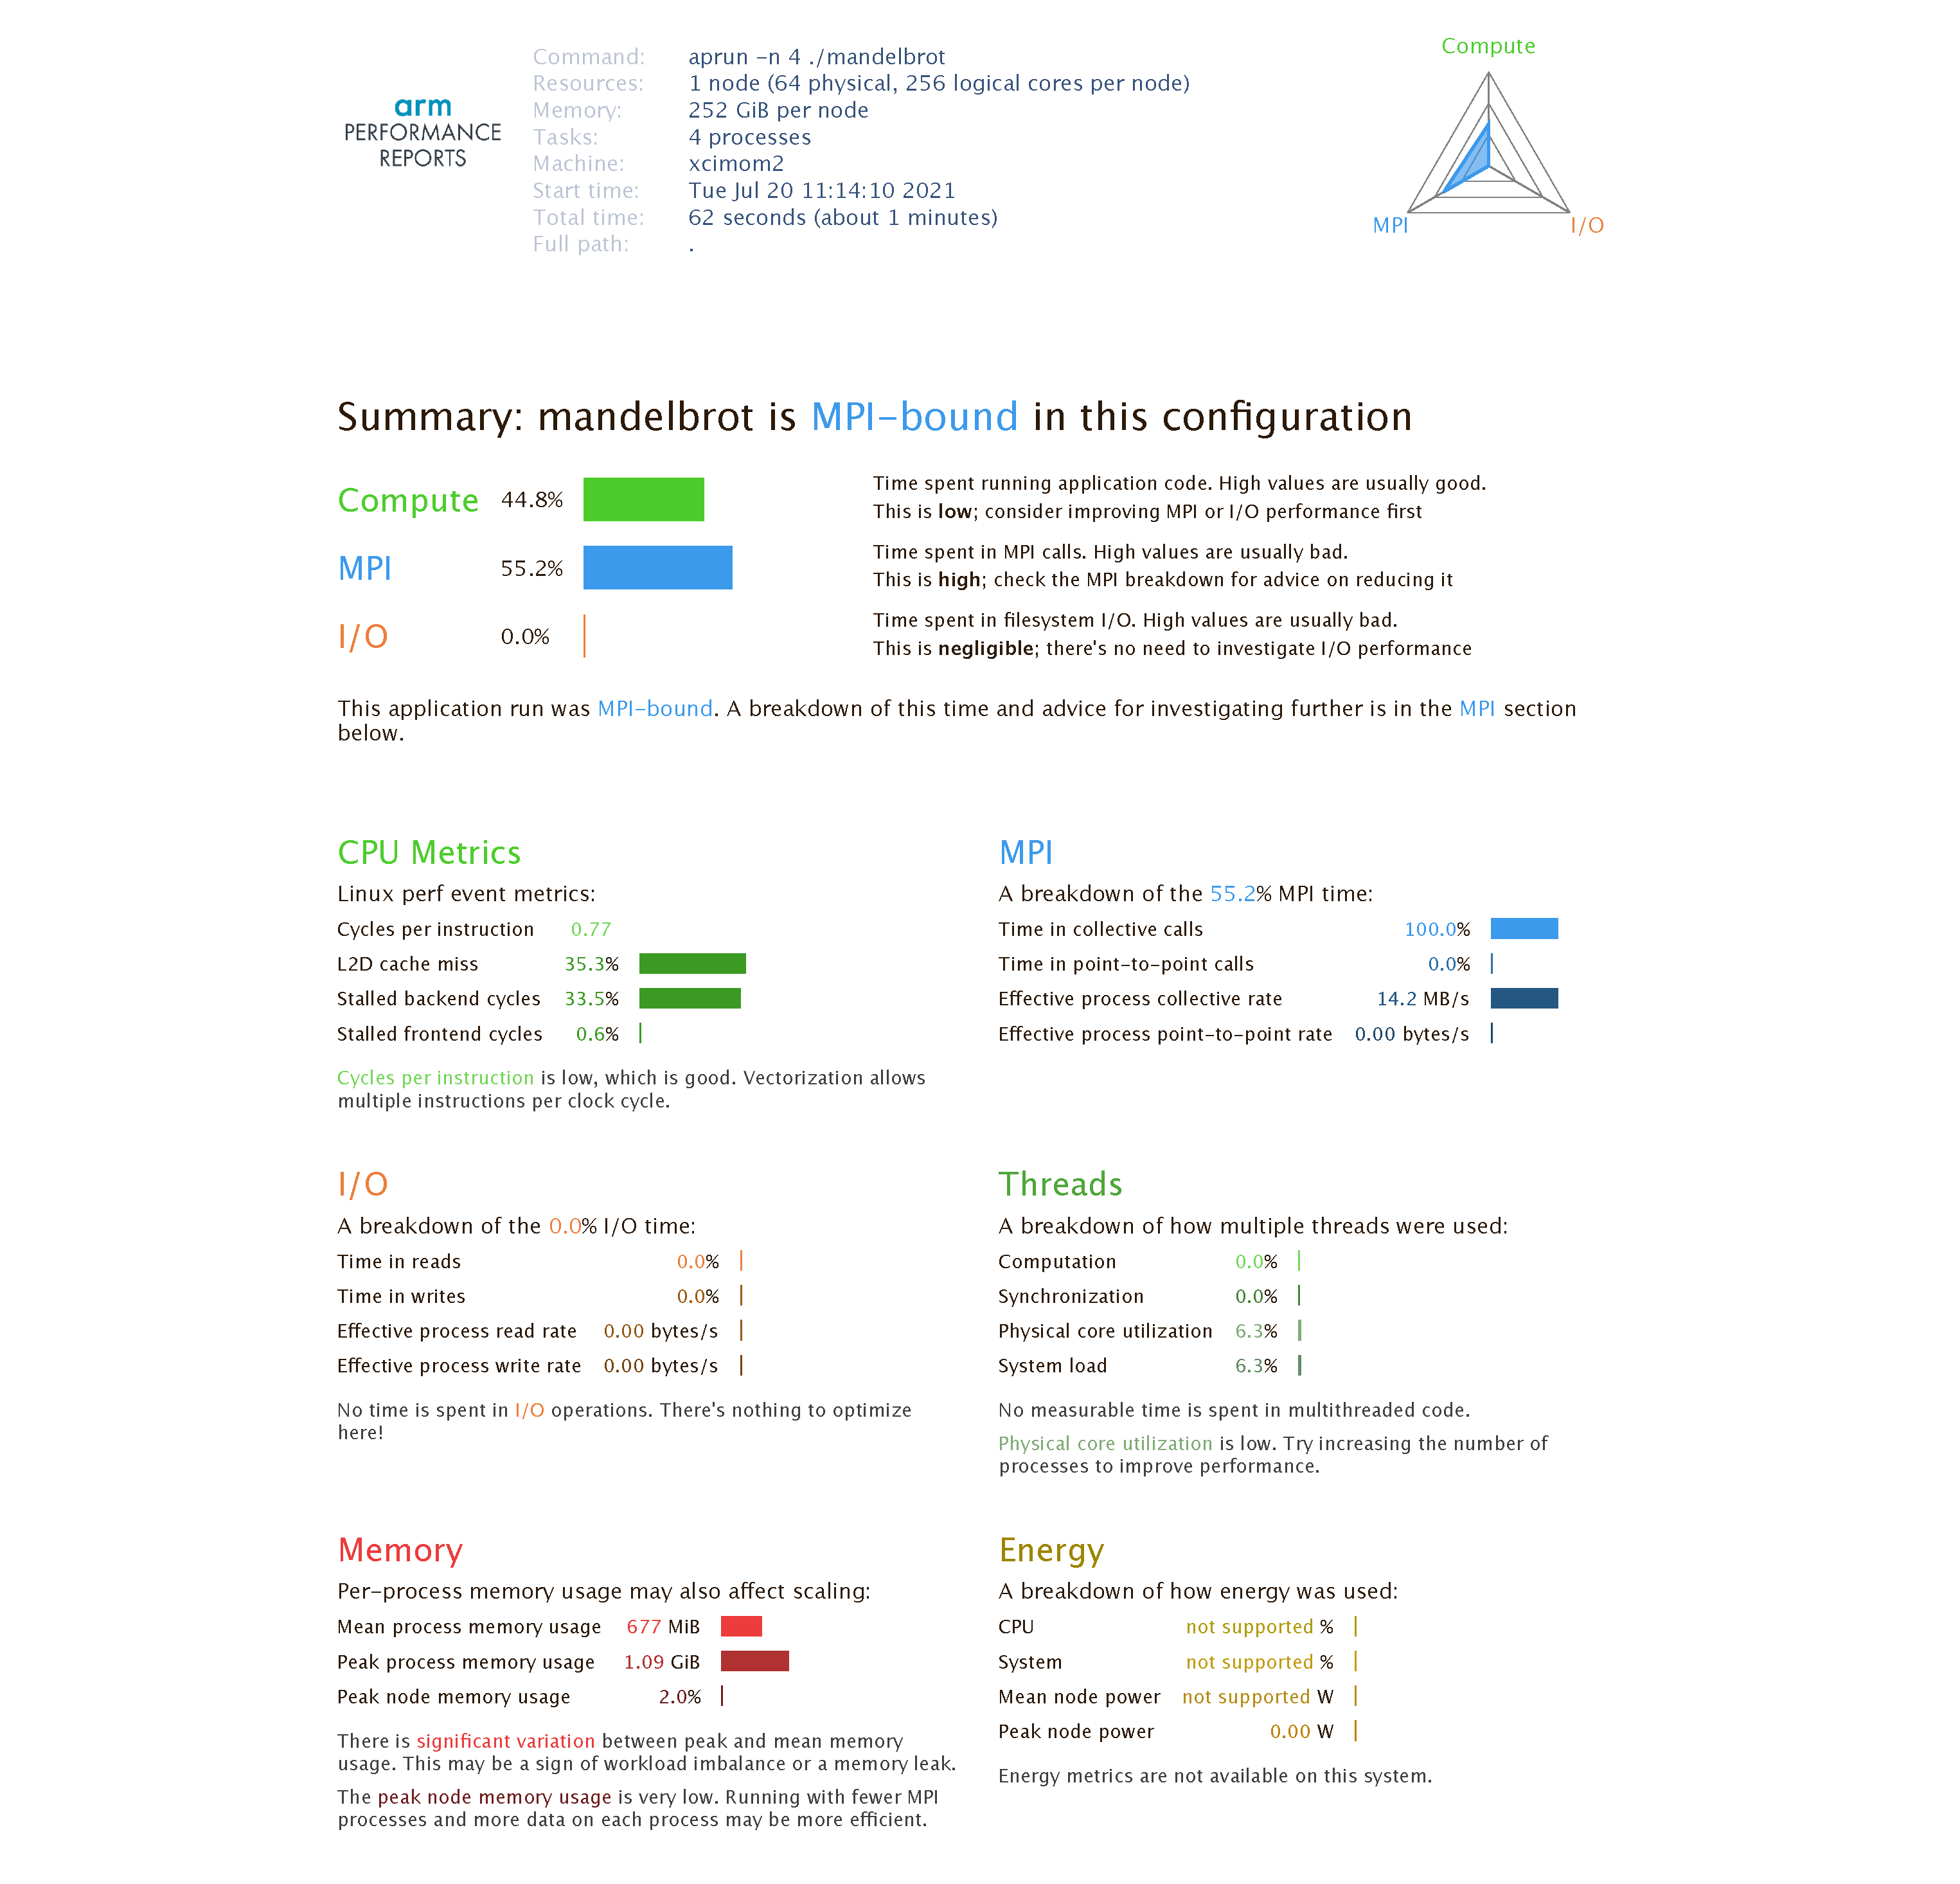
\includegraphics[scale=0.35]{figures/mandelbrot_v1_PerformanceReport}
\caption{ARM Performance Report from the Mandelbrot version 1 example. The tool correctly identifies that there is excessive time spent in MPI calls but does not identify load imbalance as the performance issue.}
\label{fig:perf-report_MB1}
\end{center}
\end{figure}
In this example the I/O has been switched off to highlight the performance issue caused by the load imbalance. The tool correctly identifies that there is excessive time spent in MPI calls but does not identify load imbalance as the performance issue. 

For the next test the I/O was switched on and the results are shown in figure~\ref{fig:perf-report_MB1_IO}.
\begin{figure}[htbp]
\begin{center}
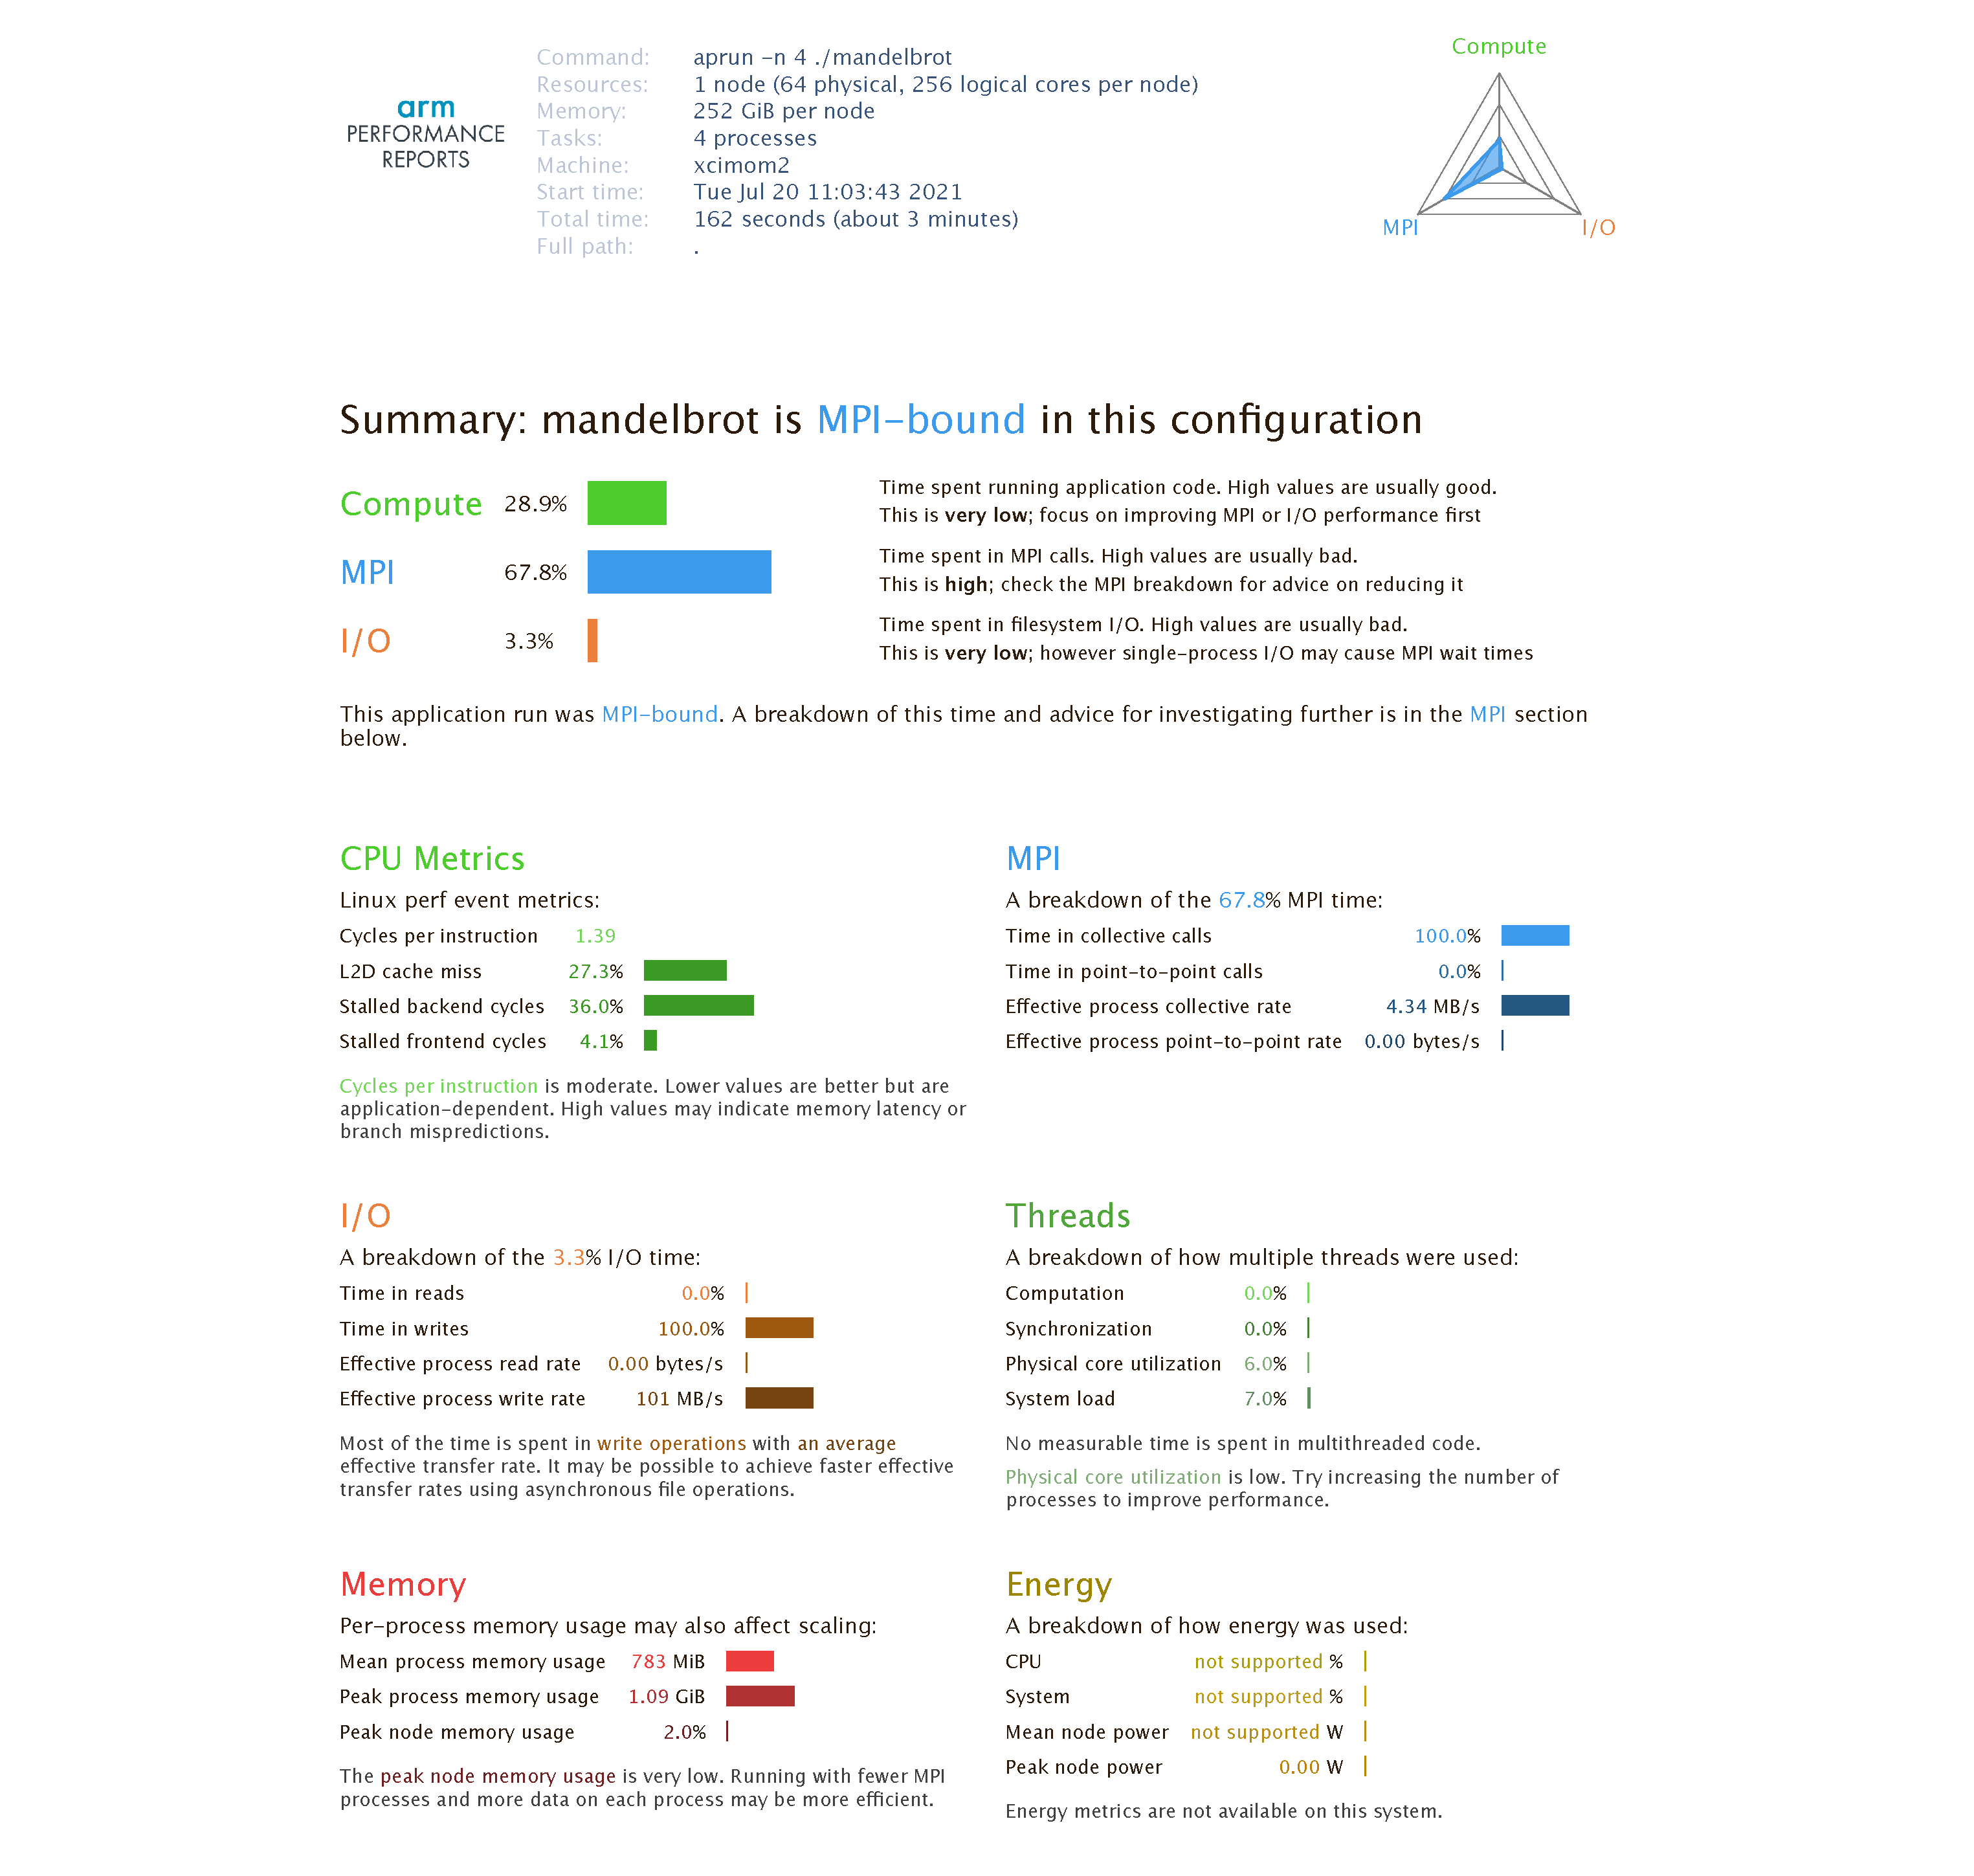
\includegraphics[scale=0.35]{figures/mandelbrot_v1_IO_PerformanceReport}
\caption{ARM Performance Report from the Mandelbrot version 1 example with I/O switched on. The additional time spent in I/O shows up as an exacerbated load imbalance due to I/O being funnelled through the rank zero process.}
\label{fig:perf-report_MB1_IO}
\end{center}
\end{figure}
The additional time spent in I/O shows up as an exacerbated load imbalance due to I/O being funnelled through the rank zero process which causes all other processes to wait at an MPI barrier. Although slow I/O is the underlying cause the time spent in I/O is only a small fraction of the time breakdown.


\begin{figure}[htbp]
\begin{center}
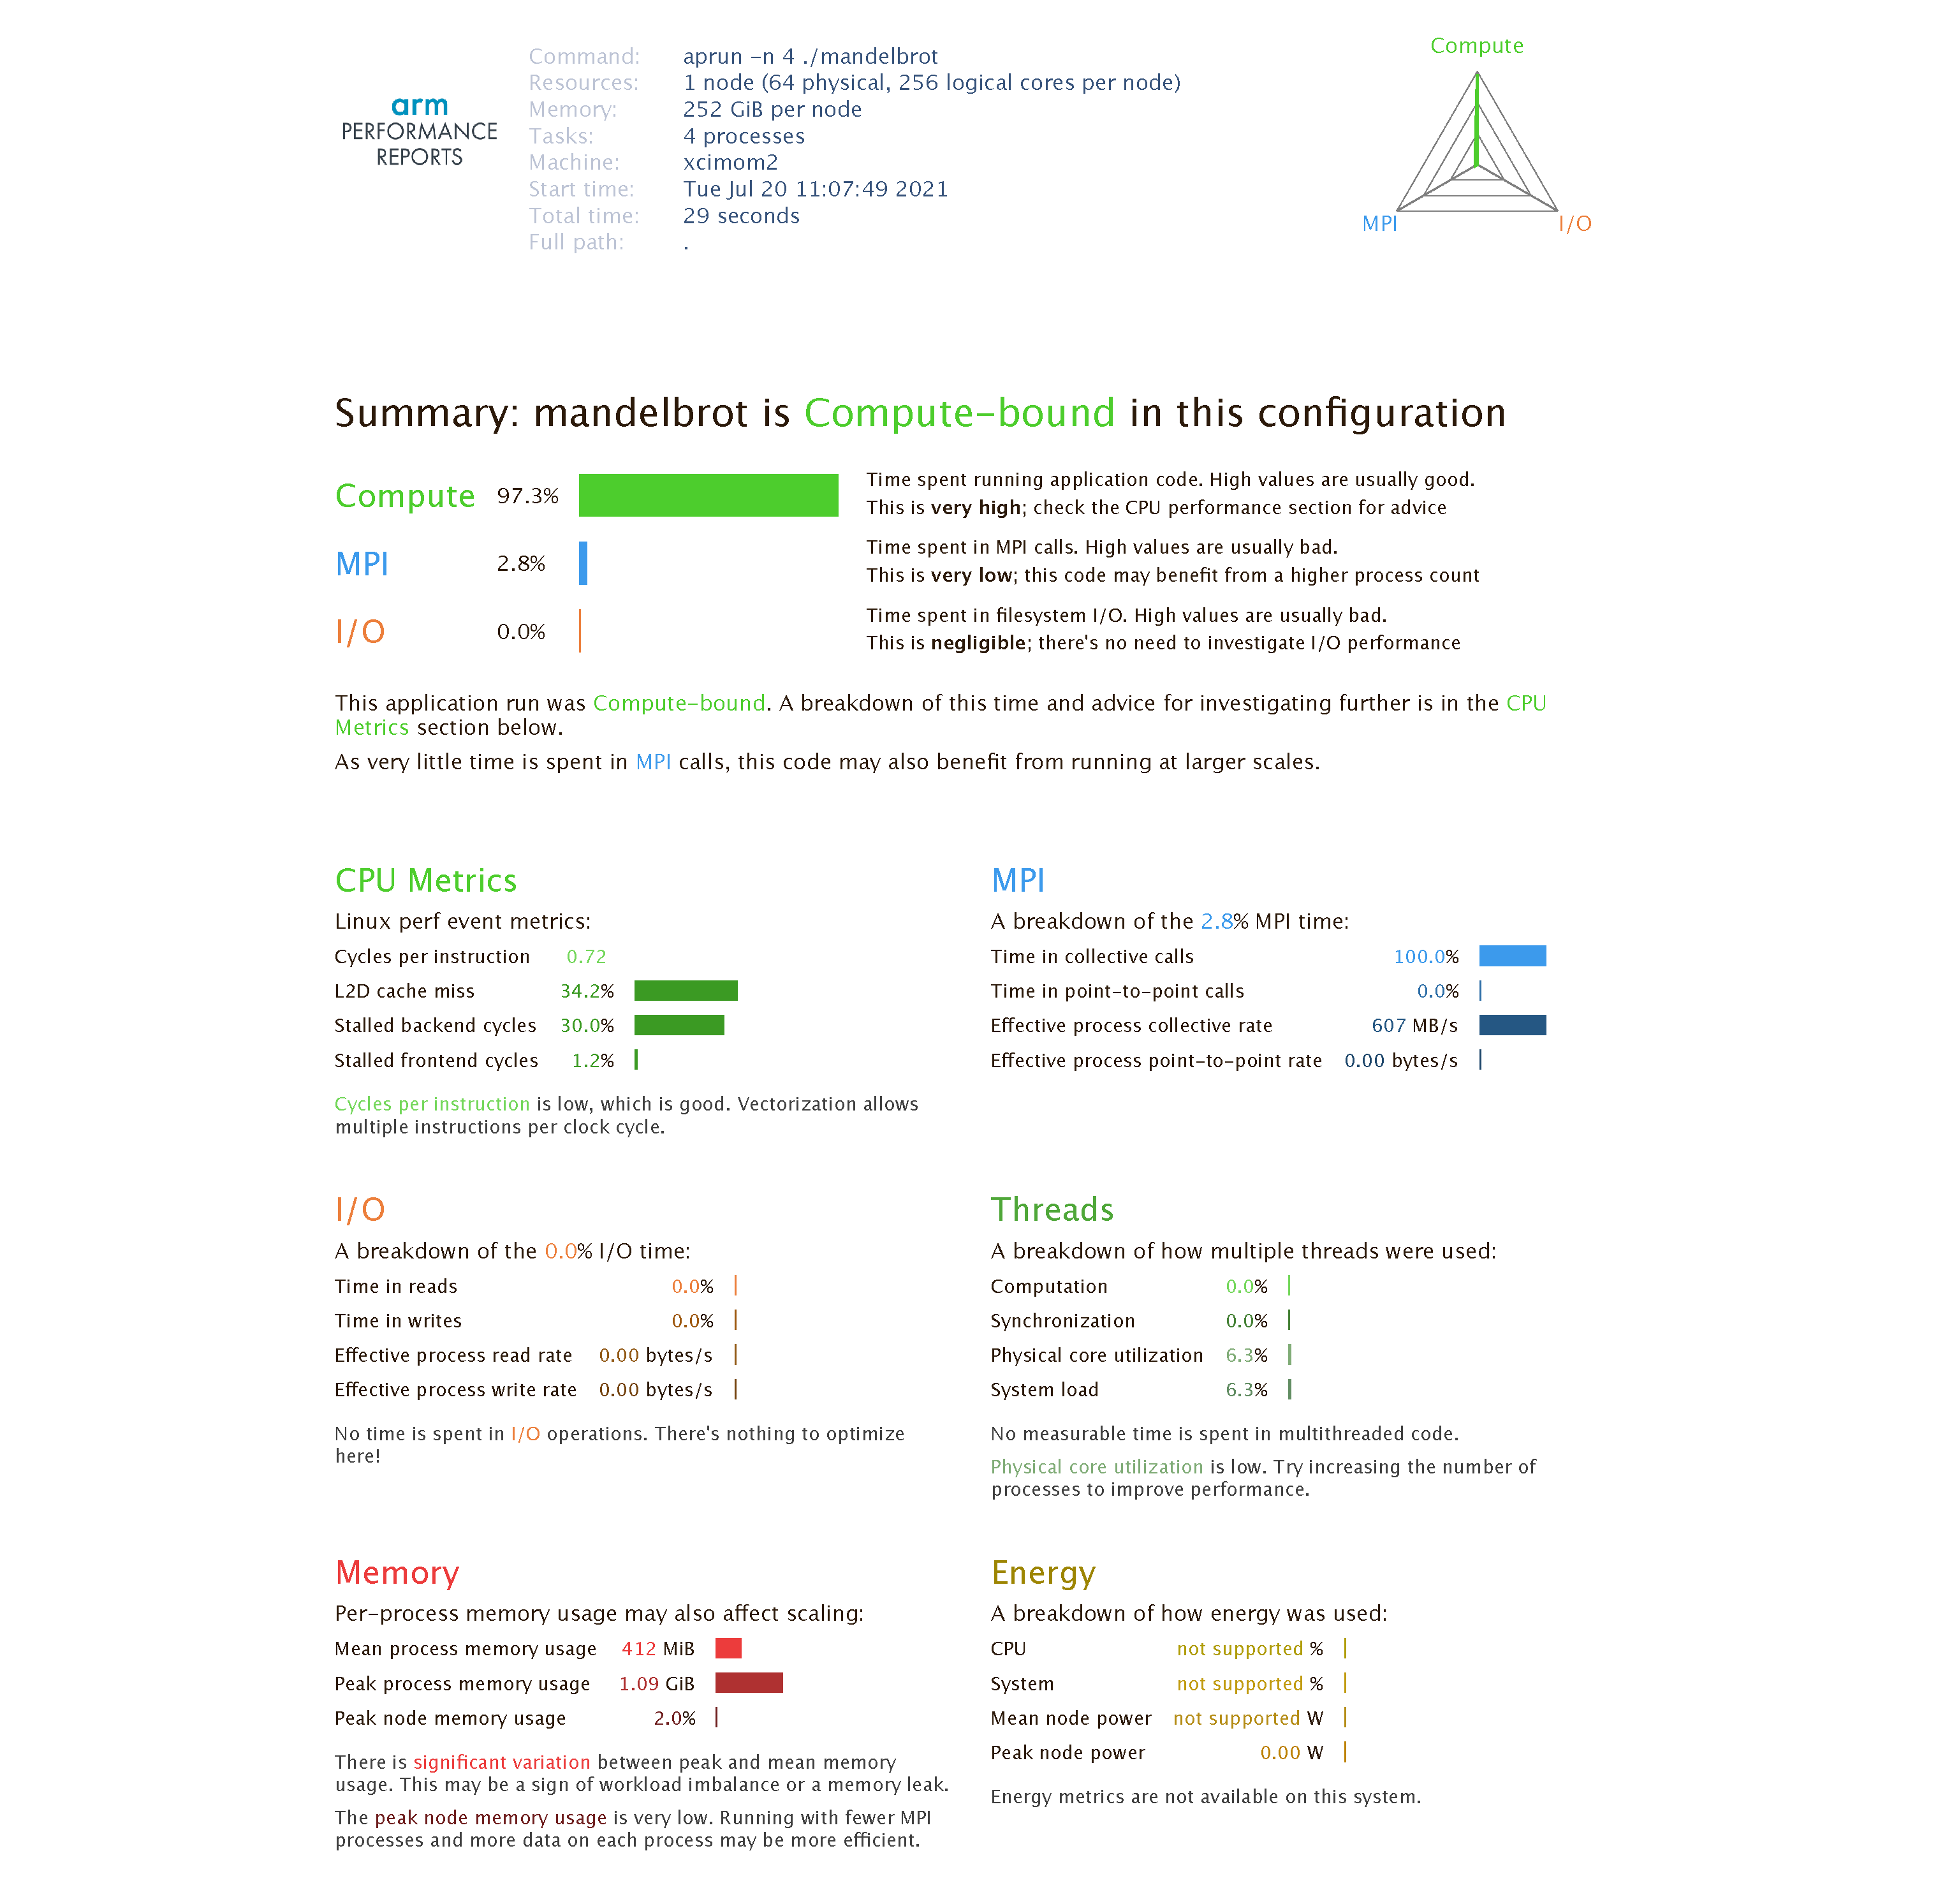
\includegraphics[scale=0.35]{figures/mandelbrot_v2_PerformanceReport}
\caption{ARM Performance Report from the Mandelbrot version 2 example. This version has fixed the load imbalance by interleaving iterations on the real axis.}
\label{fig:perf-report_MB2}
\end{center}
\end{figure}

Figure~\ref{fig:perf-report_MB3} shows the Performance Report from the Mandelbrot version 3 example with 4 MPI processes. This version of the program uses a manager-worker pattern which means that only 3 out of 4 MPI processes carry out the calculation and the fourth process is the manager which does not compute any points. The MPI time of 25\% is consistent with the manager process waiting for results from the worker processes. 
\begin{figure}[htbp]
\begin{center}
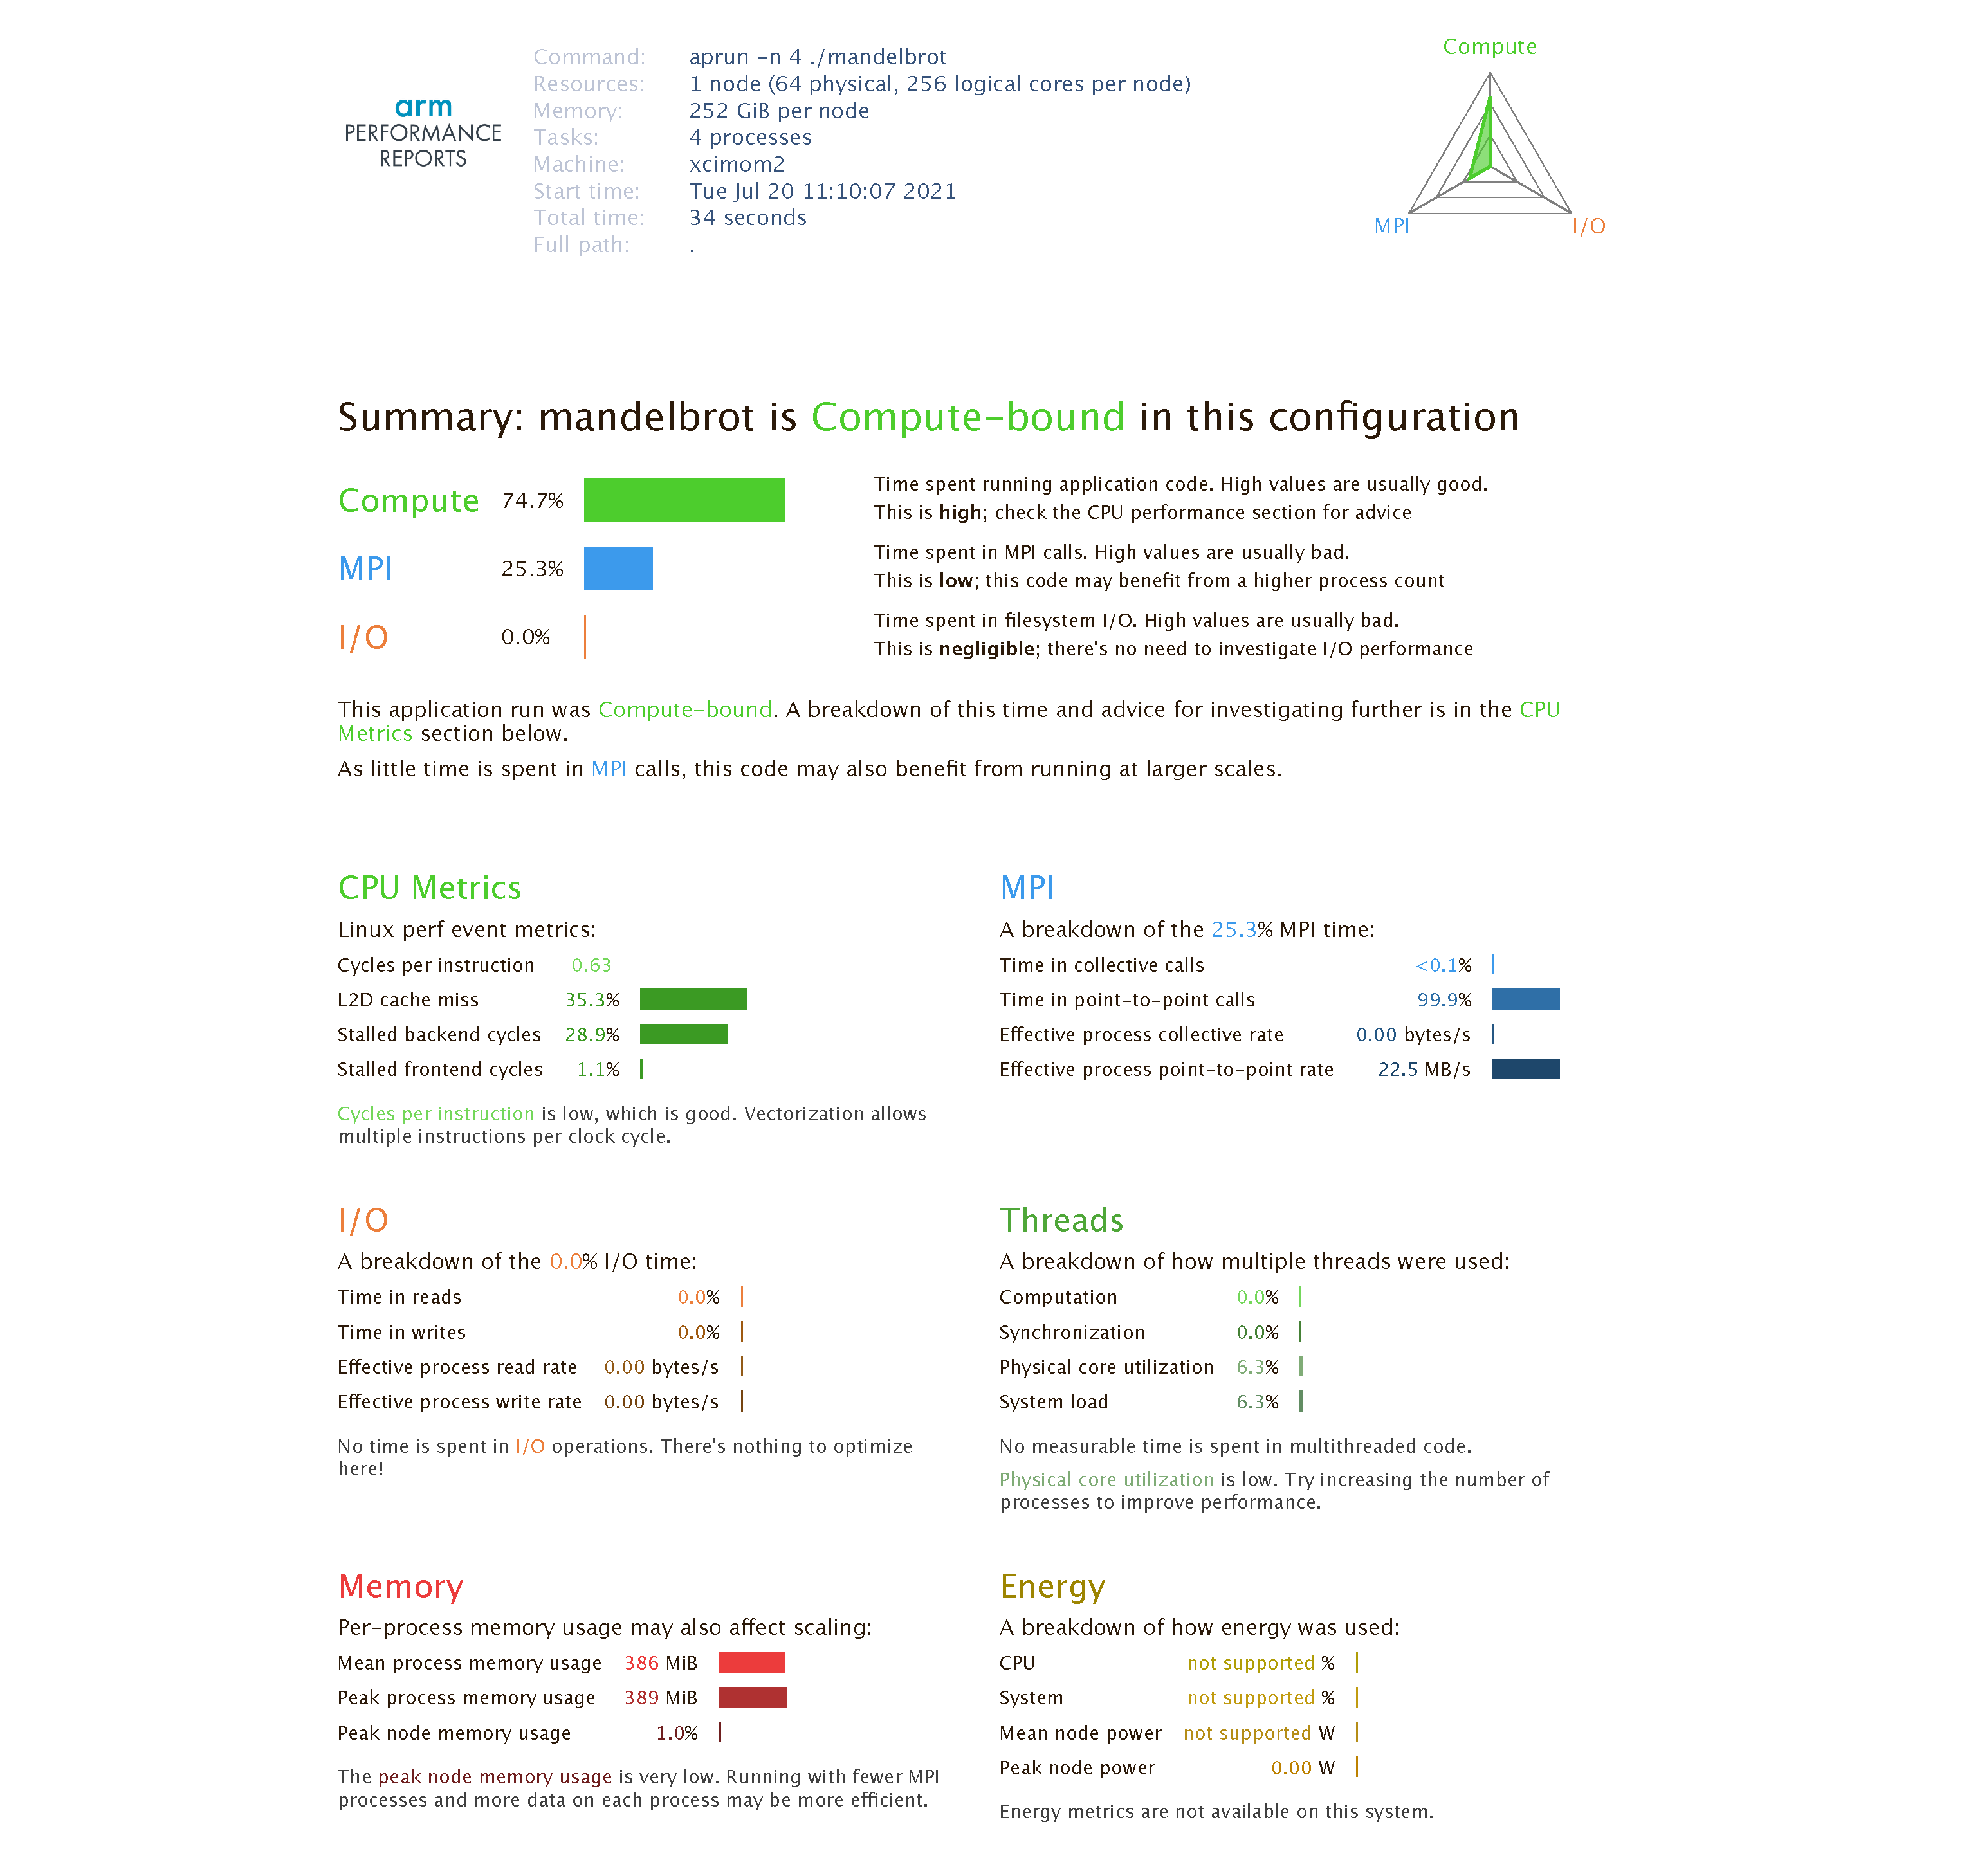
\includegraphics[scale=0.35]{figures/mandelbrot_v3_PerformanceReport}
\caption{ARM Performance Report from the Mandelbrot version 3 example with 4 MPI processes. In the manager-worker pattern only 3 out of 4 MPI processes carry out the calculation and the fourth process is the manager which does not compute any points.}
\label{fig:perf-report_MB3}
\end{center}
\end{figure}
If the number of MPI processes is increases to 16 (see figure~\ref{fig:perf-report_MB3_16procs}) then the fraction of MPI time decreases as there are now 15 processes actively working on the calculation.
\begin{figure}[htbp]
\begin{center}
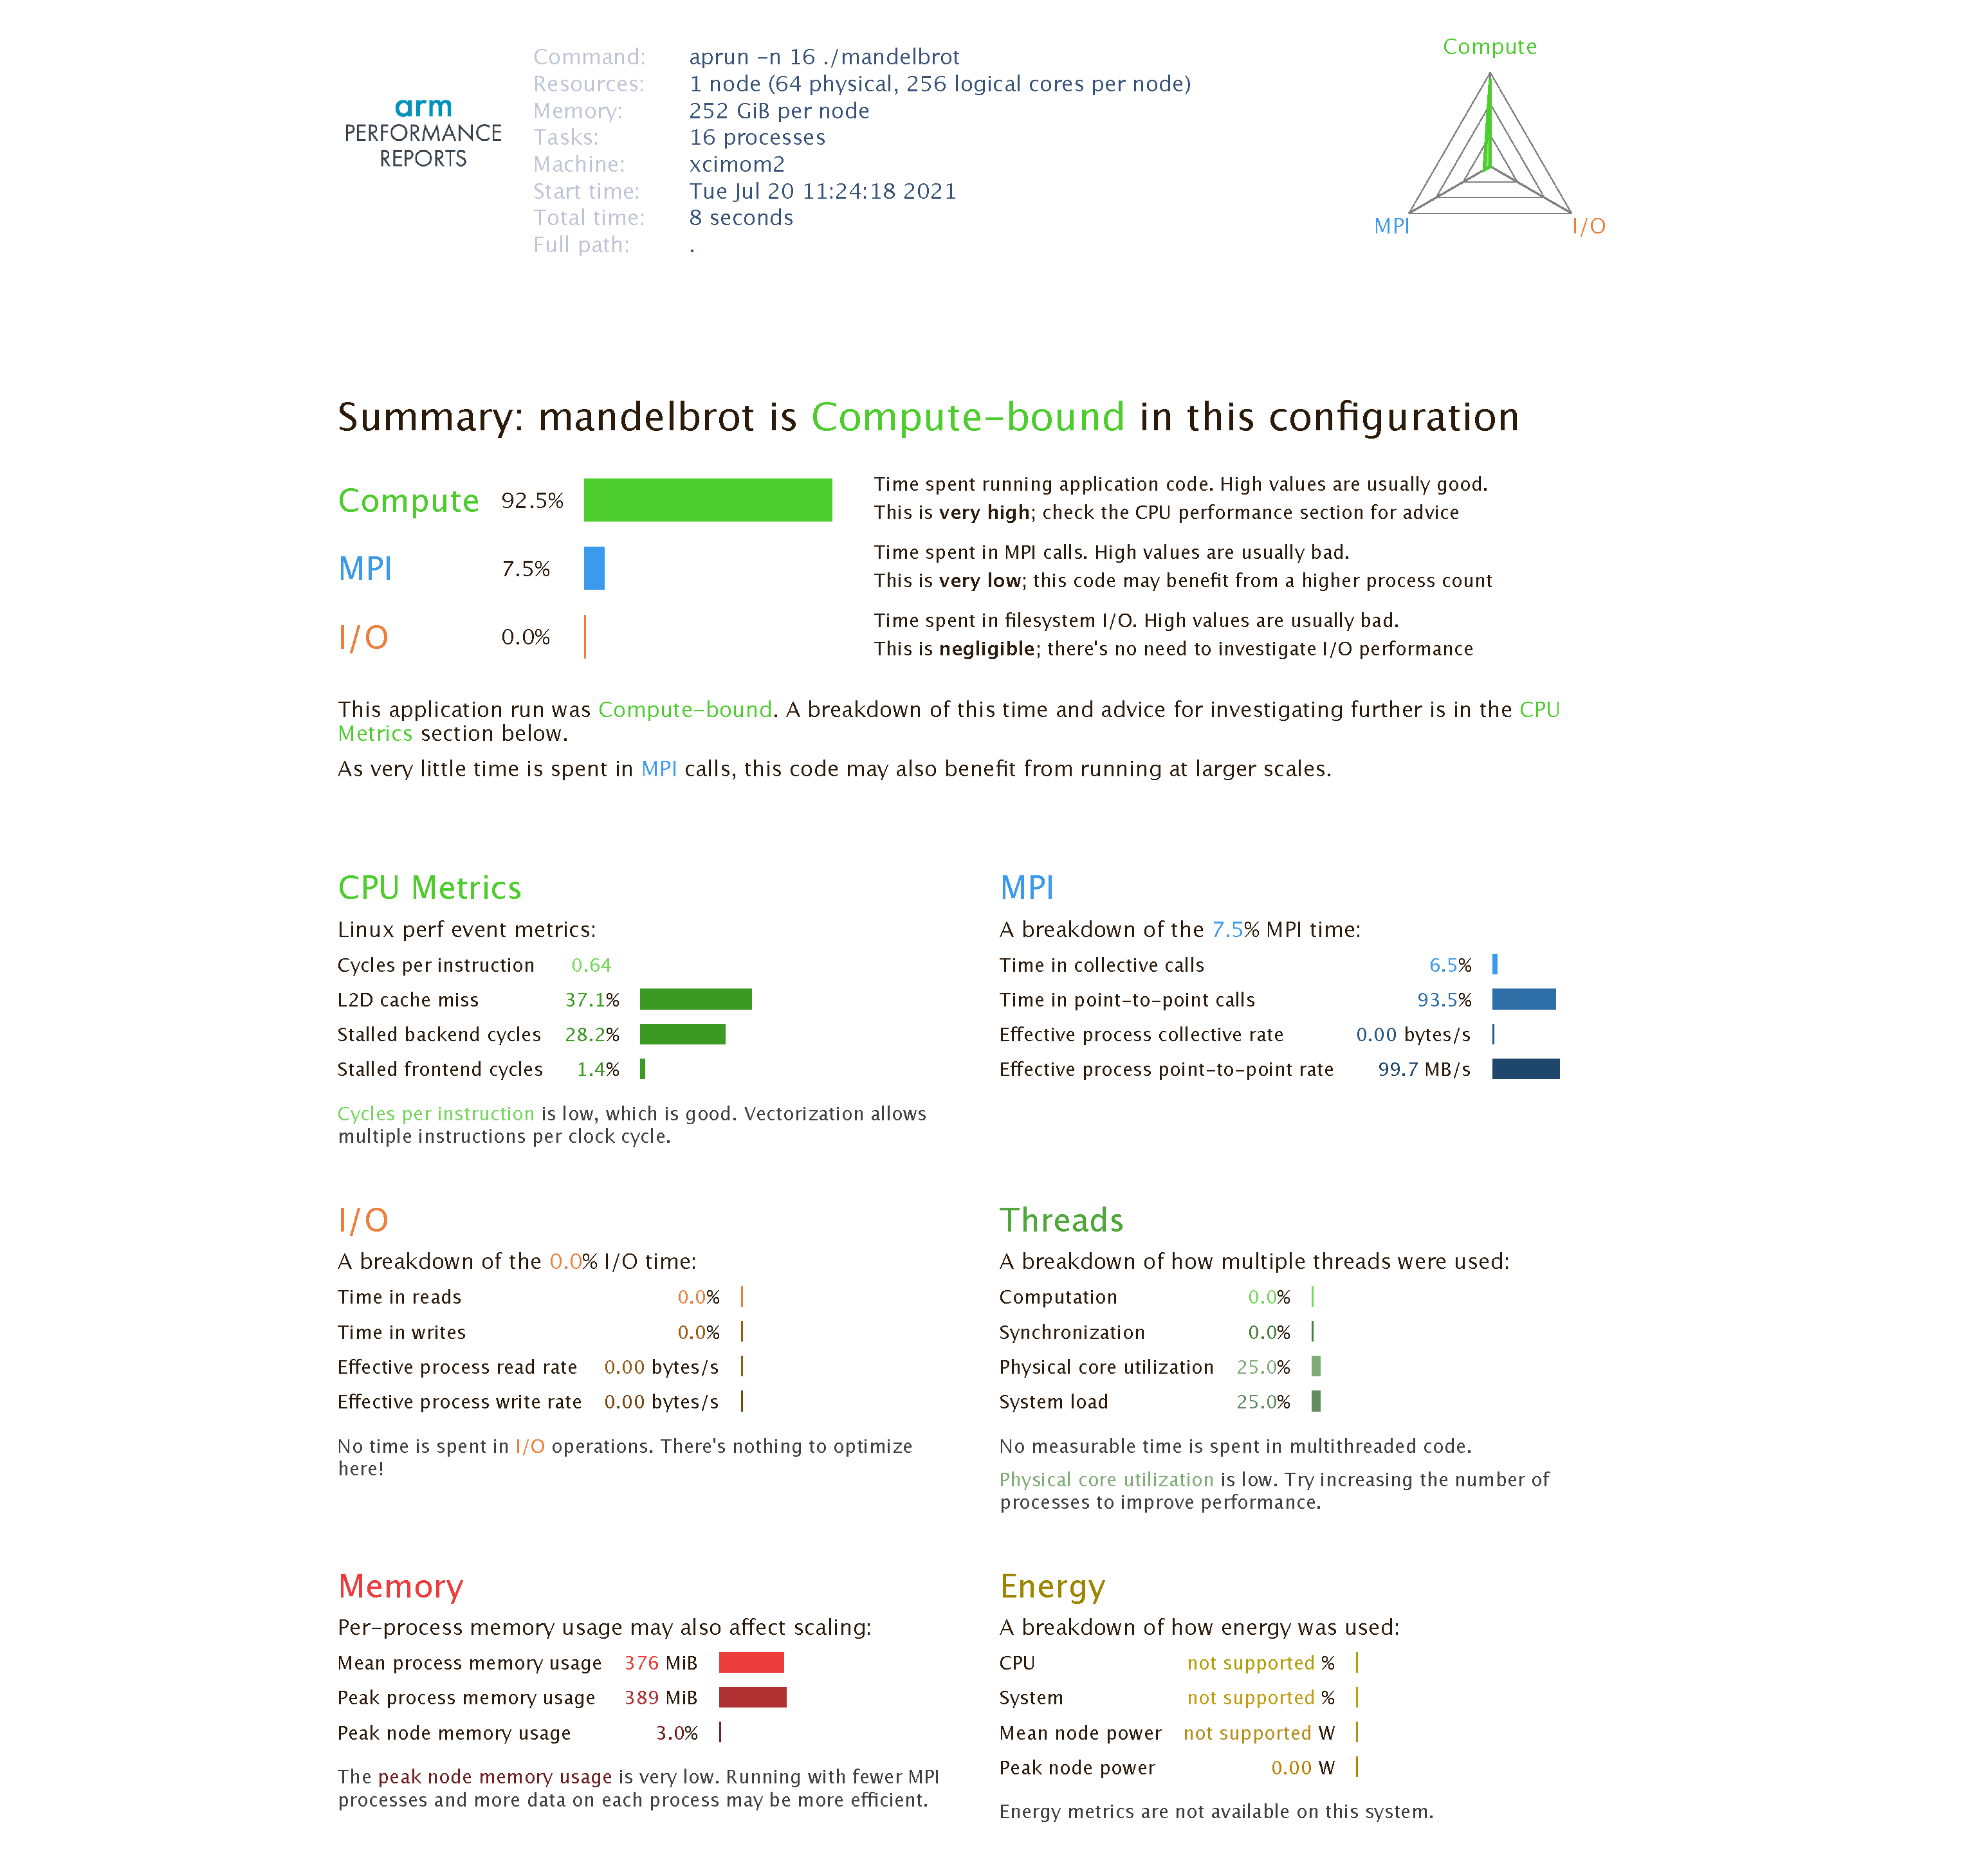
\includegraphics[scale=0.35]{figures/mandelbrot_v3_16procs_PerformanceReport}
\caption{ARM Performance Report from the Mandelbrot version 3 example with 16 MPI processes. The MPI fraction is now reduced as the manager process is only one out of 16 processes.}
\label{fig:perf-report_MB3_16procs}
\end{center}
\end{figure}

The Performance Report tool has provided a clear overview of the application performance, which highlighted the presence of performance issues, without needing to change the build process. However was not able to distinguish between load imbalance and overhead which would be clearer when viewing a time line.

%---

\subsubsection{MAP}


%---------------------------------------------------------------------------------------------------------------------

\subsection{Cray PAT}

Although this is a Cray tool it does work with compilers other than Cray (the other PrgEnv modules load perftools-base). Experience building SWIFT showed that the \texttt{perftools-lite} module can confuse autogen and configure so only load the module prior to the make command. 

\begin{itemize}
\item Cray PAT has two modes: standard and ``lite''
\item There is a graphical viewer (Apprentice 2) which reads the profiling output
\item Can view a time line from a full trace
\end{itemize}
See also \url{https://docs.nersc.gov/tools/performance/craypat/}.

It's not clear how to use Cray PAT with python/Firedrake. Loading the perftools-lite module and using the python from the cray-python module does not produce any profiling output.


%%%%%%%%%%%%%%%%%%%%%%%%%%%%%%%%%%%%%%%%%%%%%%%%%%%%%%%%%%%%%%%%%%%%%%%%%%%%%%%%%%%%%%%%%%%%%%%%%%%%%%%%%%%%%%%%%%%%%%%%%%%%%%%%%%%%%%

\section{Builds}
\label{section:builds}

There are three primary HPC platforms for the project: Isca (Exeter university Cluster), Isambard (GW4 tier-2), Archer-2 (national facility). Work on the ARCHER-2 build of Firedrake is supported by an Archer-2 eCSE project (ARCHER2-eCSE04-5 PI: Dr David A Ham (Imperial College) ``Scalable and robust Firedrake deployment on ARCHER2 and beyond'') and will not be considered further here. 

For each target platform there is a builds using the reference BLAS/Lapack implementation (fblaslapack) and optimised builds which use optimised maths libraries appropriate for the platform. The status of the builds is shown in table~\ref{table:build_status}
%
\begin{table}[htp]
\begin{center}
\begin{tabular}{|l|l|c|c|}
\hline
Platform       &  Build                   & Status         &  Profiler \\
\hline
Isca           &  GCC-OpenMPI-fblaslapack & \checkmark     &     -     \\
Isca           &  GCC-OpenMPI-OpenBLAS    & \checkmark     &     -     \\
Isambard XCI   &  GCC-CrayMPI-fblaslapack & \checkmark     & \texttt{perf-report} \\
Isambard XCI   &  GCC-CrayMPI-CrayLibsci  & \checkmark     & \texttt{perf-report} \\
\hline
\end{tabular}
\end{center}
\caption{Status of Firedrake builds and profiling for the target HPC platforms}
\label{table:build_status}
\end{table}%

\begin{itemize}
\item Flag to PETSc can be used to switch to reference version of BLAS/Lapack
\item To see how PETSc was configured see the end of the file \texttt{firedrake/src/petsc/configure.log}

\item Vendor supplied maths libraries often have support for multi-threading which needs to be switched off when using Firedrake. Newer Firedrake versions warn about this.

\item Isambard build of Firedrake: what's happening with BLAS/Lapack etc? Scalapack gets built as part of the PETSc build but is also available from \texttt{libsci}
\item Building Firedrake on Isca with the Intel compilers is not working because pybind11 requires Intel C++ compiler v18 or newer. Try pip installing pybind11 before running the Firedrake install script.
\item The Isca build scripts are named \verb+install_firedrake_isca_COMPILER_MPI_MATHLIB.sh+
\end{itemize}

%%%%%%%%%%%%%%%%%%%%%%%%%%%%%%%%%%%%%%%%%%%%%%%%%%%%%%%%%%%%%%%%%%%%%%%%%%%%%%%%%%%%%%%%%%%%%%%%%%%%%%%%%%%%%%%%%%%%%%%%%%%%%%%%%%%%%%

\section{Profiling Firedrake}
\label{section:profiling_firedrake}

ITAC was previously working on Isca with the Intel \textbf{Say how to modify the mpirun command. Can build problems be fixed with newer compiler versions?}

ARM Forge can be used to profile python applications. Make sure to add the \verb+-j 1+ flag when using ARM profilers on Isambard otherwise there can be a hang on exit\footnote{\url{https://developer.arm.com/documentation/101136/2102/Appendix/Known-issues/Arm-MAP}} (this appears to be specific to the ARM64 architecture).

\textbf{Test with a Firedrake example e.g. high resolution DG advection. This will show point-to-point communication pattern from domain decomposition.}

%%%%%%%%%%%%%%%%%%%%%%%%%%%%%%%%%%%%%%%%%%%%%%%%%%%%%%%%%%%%%%%%%%%%%%%%%%%%%%%%%%%%%%%%%%%%%%%%%%%%%%%%%%%%%%%%%%%%%%%%%%%%%%%%%%%%%%

\section{Conclusions and recommendations}
\label{section:conclusions}

Carry out initial performance studies using Firedrake for rapid prototyping. Use ARM Forge to profile Firedrake on  Isambard which enables profiling up to the 20\,992 cores. Once the scalability of the algorithm has been established on Isambard implement the algorithm in FRric and run on Archer-2 with profiling using Cray PAT. This will enable performance studies beyond 20\,000 cores.

%%%%%%%%%%%%%%%%%%%%%%%%%%%%%%%%%%%%%%%%%%%%%%%%%%%%%%%%%%%%%%%%%%%%%%%%%%%%%%%%%%%%%%%%%%%%%%%%%%%%%%%%%%%%%%%%%%%%%%%%%%%%%%%%%%%%%%

\end{document}
